% %%%%%%%%%%%%%%%%%%%%%%%%%%%%%%%%%%% %
% Template criado por @Guvidaletti    %
% Utilizando o template da AGES v2.1  %
% como base                           %
% %%%%%%%%%%%%%%%%%%%%%%%%%%%%%%%%%%% %

% Configuração do Documento
\documentclass[
  a4paper,
  12pt,
  oneside,
  chapter=TITLE,
  english,
  brazil]
  {abntex2}

\usepackage[brazil]{babel}

\usepackage[
  tmargin=3cm,
  lmargin=3cm,
  bmargin=2cm,
  rmargin=2cm,
]{geometry}


% Para utilizar imagens dentro do LaTeX:
\usepackage{graphicx}

% \usepackage{lmodern}			% Usa a fonte Latin Modern
\usepackage{helvet}             % Usa a fonte Helvetica
\usepackage[T1]{fontenc}		% Selecao de codigos de fonte.

% Para utilizar fontes diferentes:
% Define Sans Serif para todo documento
\renewcommand{\familydefault}{\sfdefault}

% Deve haver recuo no primeiro paragrafo
\usepackage{indentfirst}

% Capitulos, secoes e subsecoes devem ter tamanho normal
\renewcommand{\ABNTEXchapterfontsize}{\normalsize}
\renewcommand{\ABNTEXsectionfontsize}{\normalsize}
\renewcommand{\ABNTEXsubsectionfontsize}{\normalsize}
\renewcommand{\ABNTEXsubsubsectionfontsize}{\normalsize}

% Capitulos e secoes devem estar negritados
% https://groups.google.com/g/latex-br/c/ULm17Zfng3w/m/ZbCHIHLi7GAJ
\renewcommand{\ABNTEXchapterfont}{\normalfont\sffamily\bfseries}
\renewcommand{\ABNTEXsectionfont}{\normalfont\sffamily\bfseries}
% Subsecoes nao devem estar negritados
\renewcommand{\ABNTEXsubsectionfontsize}{\normalfont\sffamily}

% Espacamento vertical entre titulo do capitulo e conteudo deve ser de 24pts
\setlength\afterchapskip{24pt}

% Define colores para links
\hypersetup{
    colorlinks=true,
    linkcolor=black,
    citecolor=black,
    urlcolor=black,
}

% Páginas sem cabeçalho
\pagestyle{simple}

% Subseção não no sumário: (para ir, trocar para 2)
\addtocontents{toc}{\protect\setcounter{tocdepth}{1}}

% Captions com negrito
% \usepackage[font=bf]{caption}
% Caption pequena, com o "Figura" em negrito
\usepackage[font=small,labelfont=bf]{caption}

% Posicionamento de Figuras - Importantíssimo
\usepackage{float}

% Espaçamento de 1,5
\renewcommand{\baselinestretch}{1.5}


% Para a lista de abreviaturas:
\usepackage[printonlyused,withpage]{acronym}

% Se o style=abnt não funcionar, utilize o style=numeric
\usepackage[style=abnt]{biblatex}
\usepackage{csquotes}
\addbibresource{bibliografia/bibliografia.bib}

% Ajuste de ordenação dos arquivos:
\begin{document}
  \author{João Miguel}

\def\autor{\uppercase{João Miguel Bonaldo Meier}}
\def\inicio{02/2025}
\def\fim{06/2025}
\def\ages{II}
\def\local{Porto Alegre, RS}
\def\ano{2025}

\begin{capa}
  \centering
    \uppercase{
      PONTIFÍCIA UNIVERSIDADE CATÓLICA DO RIO GRANDE DO SUL\\
      ESCOLA POLITÉCNICA\\
      CURSO DE BACHARELADO EM ENGENHARIA DE SOFTWARE\\
      AGES $-$ AGÊNCIA EXPERIMENTAL DE ENGENHARIA DE SOFTWARE\\
      }

    \vfill
    \autor\\
    \vfill
    \textbf{
      \uppercase{
        Memorial de atuação na Agência Experimental de Engenharia de Software 
        {-} Período \inicio\ a \fim\
        \\AGES \ages\
      }
    }
    
    \vfill

    \vfill
    \local\\
    \ano\
  \end{capa}
  % Opcional:
  \def\textoDedicatoria{
  Dedicatória: Texto no qual o autor
  do trabalho oferece homenagem ou
  dedica o seu trabalho a alguém.
}

\begin{dedicatoria}
  \textbf{Dedicatória}
  \vfill
  % Dedicatória:
  \hfill{}
  \parbox{6cm}{
    \begin{flushright}
      \textoDedicatoria\
    \end{flushright}
      }
\end{dedicatoria}
  % Opcional:
  \begin{agradecimentos}[\protect\bfseries Agradecimentos]
  % Agradecimentos - Inicio
  Os agradecimentos devem ser dirigidos àqueles que contribuíram de maneira
relevante à elaboração do trabalho, restringindo-se ao mínimo necessário, como
instituições (CNPq, CAPES, PUCRS, empresas ou organizações que fizeram parte
da pesquisa), ou pessoas (profissionais, pesquisadores, orientadores, etc.).

Os agradecimentos devem ser colocados de forma hierárquica de importância
e para trabalhos financiados com recursos de instituições (CAPES, CNPq, FINEP,
FAPERGS, etc.) os agradecimentos são obrigatórios a essas instituições.
  % Agradecimentos - Fim
\vfill
\end{agradecimentos}
  % Opcional:
  \def\textoEpigrafe{
Se continuar fazendo o que sempre fez, vai continuar obtendo
o que sempre obteve
}

\def\autorEpigrafe{Jessie Potter}

\begin{epigrafe}
  \vspace*{\fill}
  \hfill{}
  \parbox{6cm}{
    \begin{flushright}
      % Epígrafe - Inicio
      \textit{``\textoEpigrafe``}\\
      \bigbreak\
      % Epígrafe - Fim
      \textbf{\autorEpigrafe}
  
    \end{flushright}
  }
\end{epigrafe}
  \begin{resumo}[\protect\bfseries Resumo]
Este artigo visa apresentar a trajetória de João Miguel Bonaldo Meier ao longo de suas atividades, vivências e aprendizados na AGES, uma disciplina prática dividida em quatro etapas, integrante do currículo de Engenharia de Software da Pontifícia Universidade Católica do Rio Grande do Sul. Serão expostas as principais atividades do projeto desenvolvido durante a AGES I e AGES II, realizada pelo autor, destacando-se o que foi realizado nas Sprints 0 e 1, bem como os aprendizados e conclusões relacionadas a esta experiência até o momento atual.
  \bigbreak\
  \\\textbf{PALAVRAS CHAVES:}
AGES, Engenharia de Software, Pontifícia Universidade Católica do Rio Grande do Sul, Aprendizados, Experiência Prática.
\end{resumo}
  \listoffigures*
  \listoftables*
  % forma de utilizar no texto:
% \ac{ages} << exemplo

\begin{center}
  \uppercase{\bfseries lista de siglas}\\[3em]
\end{center}

\begin{acronym}[XXXXXXXX]
  % Só vai aparecer no texto se for utilizado
  % \acro{acronym}[short name]{full name}
  \acro{ages}[AGES]{Agência Experimental de Engenharia de Software}
  \acro{us} [US] {User Story}
  \acro{sql} [SQL] {Structured Query Language}
  \acro{bd} [BD] {Banco de Dados}
  \acro{ssr} [SSR] {Server Side Rendering}
  \acro{http} [HTTP] {Hypertext Transfer Protocol}
  \acro{rest} [REST] {Representational State Transfer}
  \acro{api} [API] {Application Programming Interface}
  \acro{cicd} [CI/CD] {Continuous Integration Continuous Delivery}
  \acro{pucrs} [PUCRS] {Pontifícia Universidade Católica do Rio Grande do Sul}
\end{acronym}
  \tableofcontents*

  % Contagem de páginas começa aqui:
  \textual{}
  % ajuste pare remover cabeçalho:
  % verificar se não é melhor com
  \pagestyle{simple}

  % Capitulos
  \chapter[APRESENTAÇÃO DA TRAJETÓRIA DO ALUNO]{APRESENTAÇÃO DA TRAJETÓRIA DO ALUNO}

Desde 2023, João Miguel Bonaldo Meier é graduando em Engenharia de Software. Seu primeiro contato com programação ocorreu em 2017, durante um curso técnico em informática. Já na universidade, em maio de 2023, teve sua iniciação acadêmica no PET Informática, onde se envolveu com tarefas de pesquisa científica e extensão. No mesmo ano, conquistou uma vaga de estágio em Automação Fiscal na Dell Technologies. Durante esse período, adquiriu conhecimentos em tecnologias como Python, SQL e Power BI, além de conceitos financeiros e desenvolveu habilidades interpessoais, como pensamento organizacional, responsabilidade, comunicação, liderança e trabalho em equipe.

Em 2024, João iniciou a AGES I, uma prática integrada ao seu curso, com o projeto "LET ME TRIAL". Este desafio o colocou frente a conceitos complexos de software que vão além do ensino formal até o terceiro semestre. Sem um amplo conhecimento técnico prévio, além do obtido em disciplinas como Algoritmos e Estruturas de Dados, Programação Orientada a Objetos, e Gerenciamento e Configuração de Software, João vem desenvolvendo habilidades técnicas avançadas em Java SpringBoot, bibliotecas de testes unitários, como Mockito, além de outras ferramentas usadas em todo o processo de desenvolvimento de software, como: Docker, Figma, e conceitos de arquitetura de software.

Em maio de 2024, João mudou para outro time dentro da Dell Technologies, passando a atuar como Estagiário de Engenharia de Software. Neste novo papel, focou em desenvolvimento Salesforce (Apex), além de trabalhar com HTML, CSS, JavaScript e o framework Lightning Web Components (LWC). Além disso, ganhou experiência com GitLab CI/CD, pipelines e scripts Shell, ao construir uma pipeline de deploy para seu time de Salesforce.


Utilize referências também, modificando o arquivo \textit{bibliografia/bibliografia.bib} e citando-os com o comando\cite{artigo}.
    
  \chapter[AGES I --- “LET ME TRIAL 2024/1”]{AGES I --- “LET ME TRIAL 2024/1”}

\section[Introdução]{Introdução}

O projeto de desenvolvimento do dashboard para a Polícia Civil foi realizado durante o semestre de 2025/1, com reuniões regulares nas terças-feiras e quintas-feiras, das 17h30 às 19h00, com o objetivo de atender à necessidade de centralizar e analisar dados operacionais e administrativos de maneira eficiente. Este projeto visa criar uma solução para a visualização de dados em tempo real, permitindo uma gestão mais ágil e eficaz para os gestores da Polícia Civil, como o Chefe de Polícia e os Diretores de Departamentos. \\
A proposta surge da necessidade de integrar dados de diferentes departamentos, divisões e delegacias da Polícia Civil, oferecendo uma visão abrangente das operações e desempenho dos agentes. Atualmente, há uma dificuldade na visualização e interpretação desses dados, impactando a rapidez nas tomadas de decisão. Com a criação deste dashboard, será possível analisar indicadores como produtividade, número de ocorrências, tempo de resolução e desempenho dos agentes, melhorando a eficácia das ações e intervenções da polícia. \\
O sistema será acessível por navegadores web e dispositivos móveis, oferecendo flexibilidade e mobilidade aos gestores. O dashboard terá funcionalidades como visualizações gráficas dinâmicas, filtros personalizados e alertas em tempo real, proporcionando uma ferramenta essencial para a gestão estratégica e operacional da Polícia Civil. \\
O projeto será conduzido de acordo com a metodologia ágil, com encontros periódicos com os stakeholders, para garantir alinhamento contínuo entre as expectativas do cliente e os resultados alcançados. A seguir, a duração detalhada de cada Sprint será apresentada, ilustrando o planejamento do trabalho e os marcos atingidos ao longo do projeto.

\begin{table}[H]
    \centering
    \caption{Período de cada Sprint - AGES II}
    \begin{tabular}{|c|c|}
        \hline
        \textbf{Sprints} & \textbf{Período} \\
        \hline
        0 & 08/03/2024 a 22/03/2024\\
        1 & 22/03/2024 a 19/04/2024 \\
        2 & 119/04/2024 a 10/05/2024 \\
        3 & 10/05/2024 a 31/05/2024 \\
        4 & 31/05/2024 a 21/06/2024 \\
        \hline
    \end{tabular}
\end{table}

Este projeto foi desenvolvido sob a orientação do professor Dilnei Venturini. A equipe responsável pelo projeto ’Dashboard para a Polícia Civil’ está retratada na Figura 2.


\begin{figure}[H]
    \centering
    \small
    \caption{Time responsável pelo projeto}
    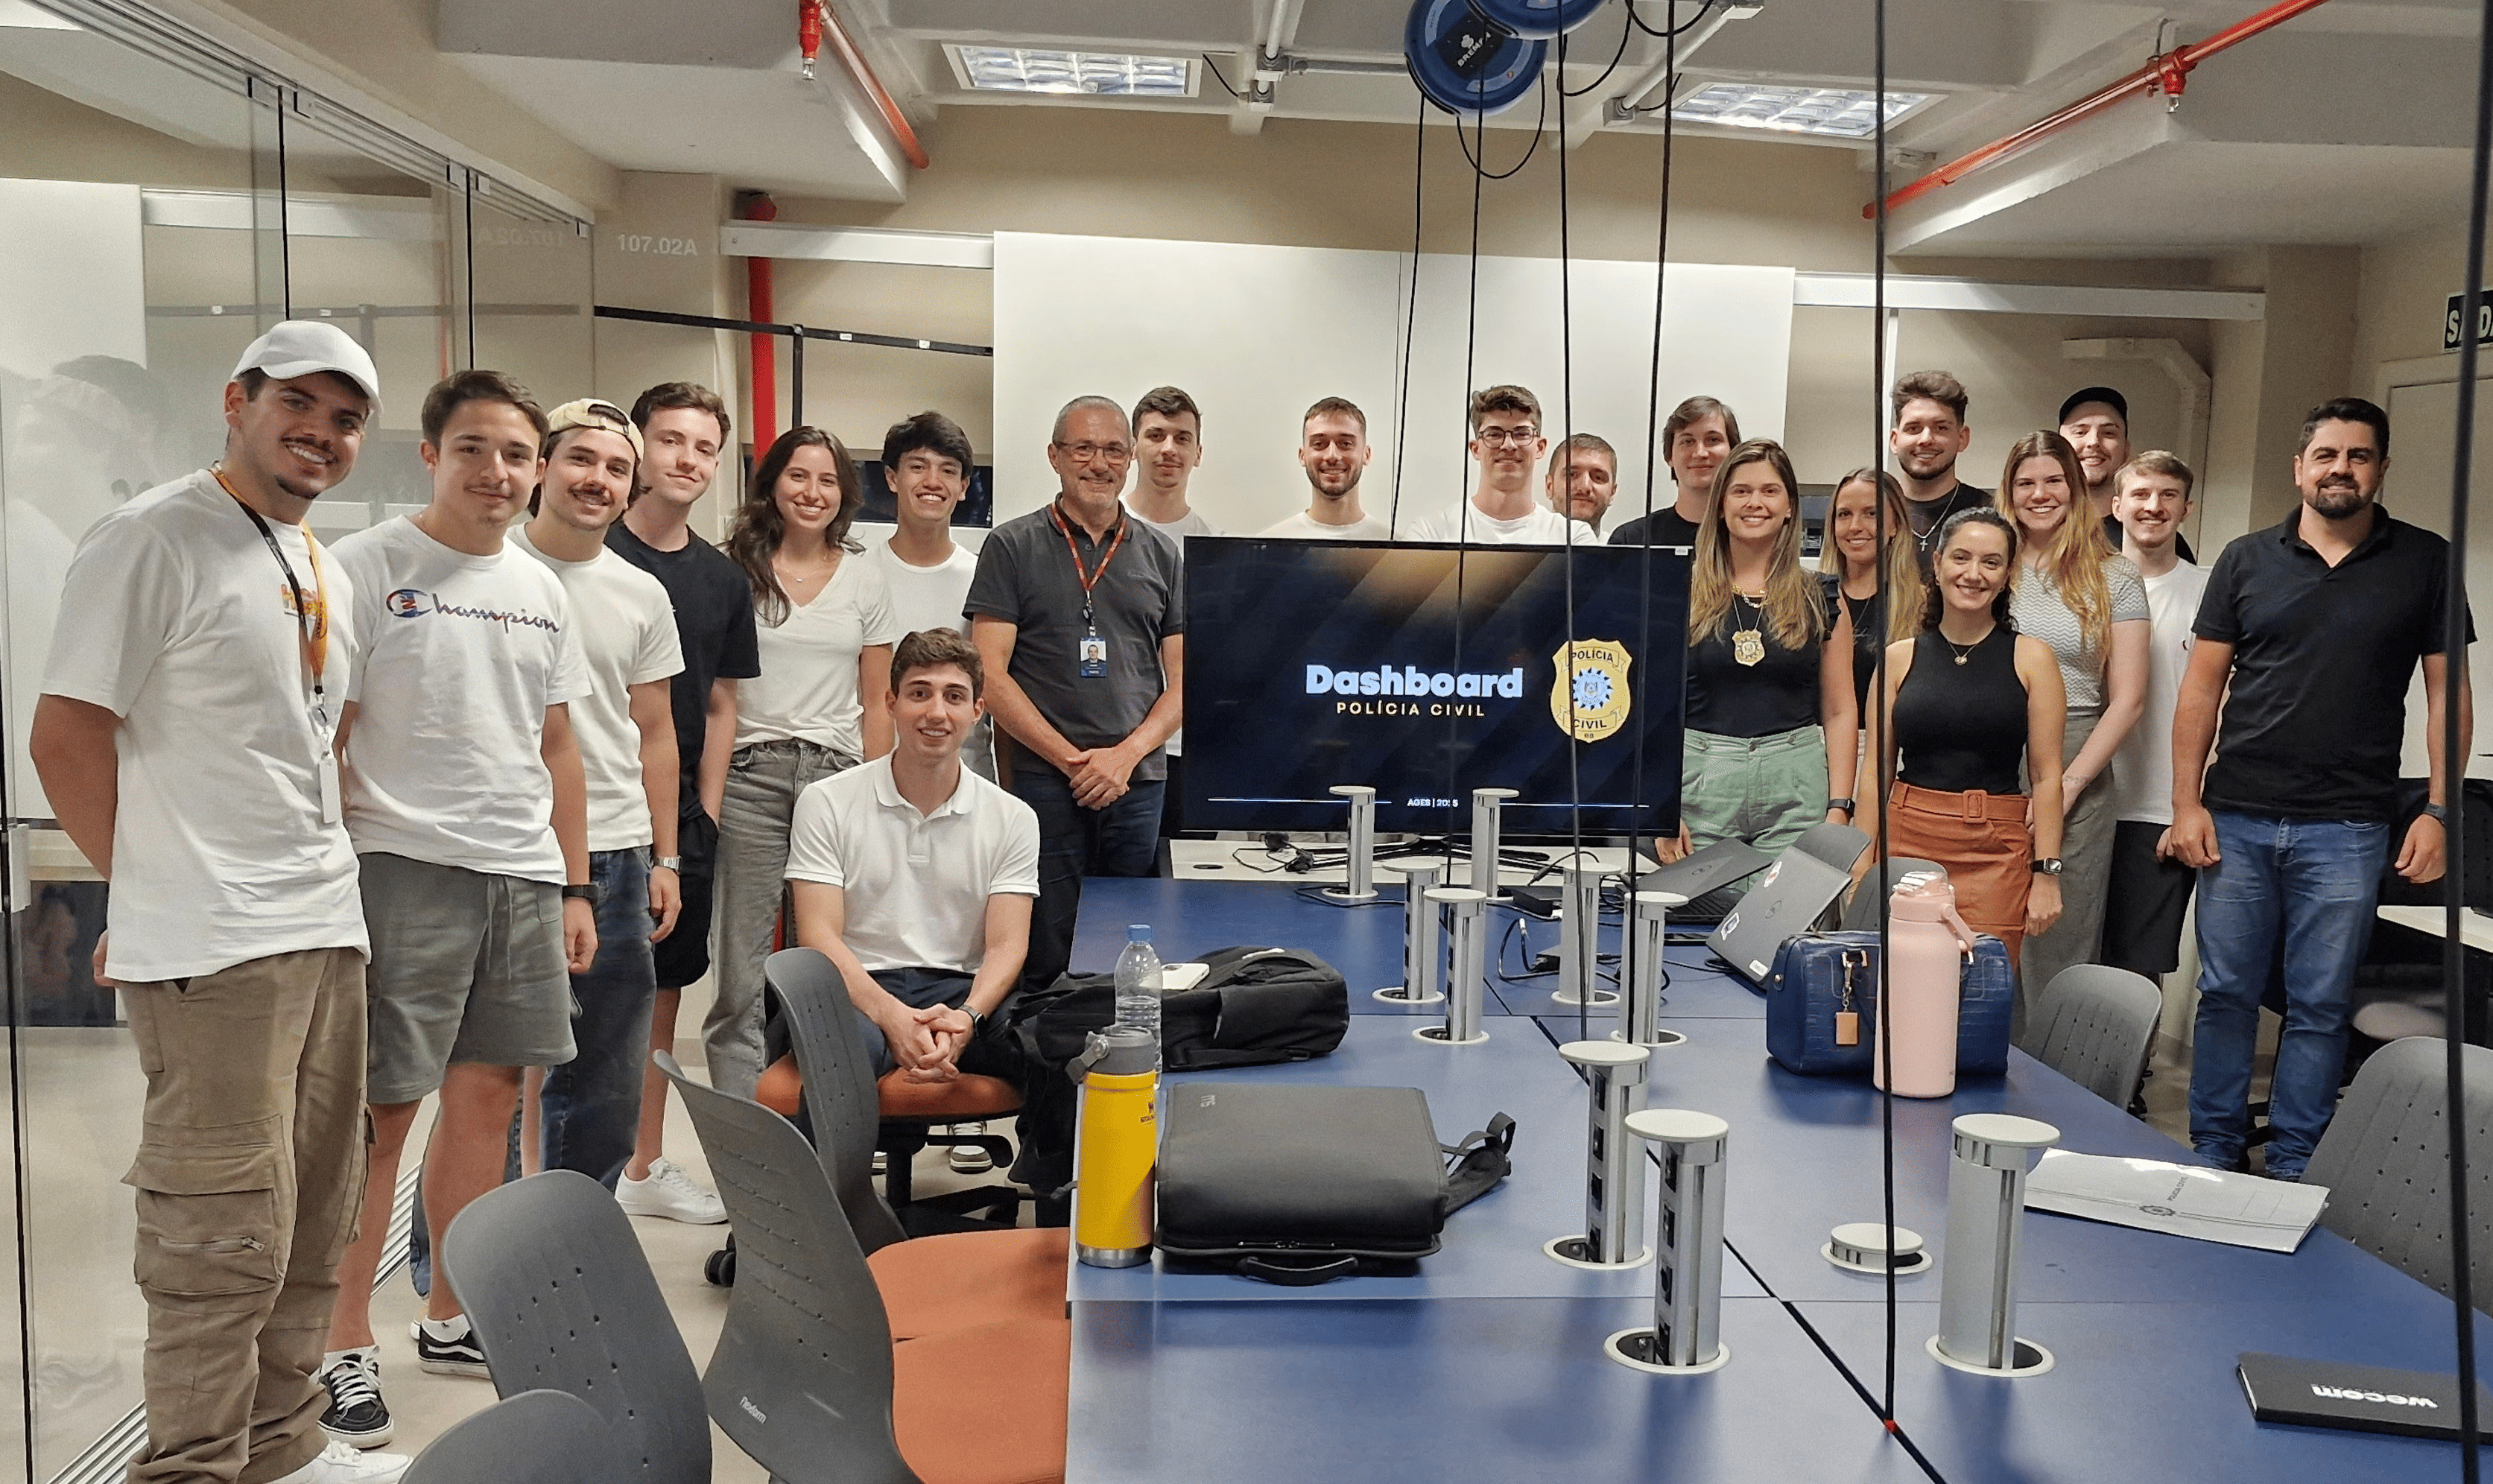
\includegraphics[width=1\linewidth]{conteudo/3 - ages II/conteudo/figures/equipe-policia-civil.png}
    \textit{Fonte: Wiki do Projeto}
    \label{fig:projeto-time}
\end{figure}
\section[Desenvolvimento do Projeto]{Desenvolvimento do Projeto}



\subsection*{Repositório do Código Fonte do Projeto}
    Um repositório público foi estabelecido no GitLab da AGES, abrangendo sete componentes distintos: api-auth, api-medico, infraestrutura, web-administrador, web- médico, web-site e uma seção dedicada à documentação no formato de Wiki.

    Para mais detalhes, consulte este link:
    {\url{https://tools.ages.pucrs.br/let-me-trial}}.


\subsection{Banco de Dados Utilizado}
  O banco de dados escolhido para o projeto foi do tipo relacional. Utilizamos PostgreSQL devido aos recursos avançados, como transações ACID (Atomicidade, Consistência, Isolamento e Durabilidade). Na \texttt{\href{http://example.com}{wiki}} do repositório, há uma seção dedicada ao banco de dados (BD), onde está detalhada toda a estrutura utilizada no projeto. Você pode visualizar o modelo conceitual completo do banco de dados na figura abaixo.


\subsection{Arquitetura Utilizada}
  Como arquitetura para o projeto, foi escolhida a arquitetura hexagonal. A arquitetura hexagonal, também conhecida como arquitetura ports and adapters, é um padrão de arquitetura de software que promove a separação clara entre a lógica de negócios e os detalhes de implementação técnica. Ela facilita a modularidade, testabilidade e manutenção do sistema, ao permitir a substituição fácil de componentes externos e a reutilização de lógicas de negócio em diferentes contextos.\\
    Na wiki do repositório, há uma seção dedicada à Arquitetura que detalha a estrutura completa. Um diagrama de alto nível ilustrando essa arquitetura pode ser encontrado na figura abaixo.


\subsection{Protótipos das Telas Desenvolvidas}
  Deverão ser apresentados os links da Wiki, com uma breve descrição.

\subsection{Tecnologias Utilizadas}
  Para o desenvolvimento do frontend, utilizamos as seguintes tecnologias principais:\\
React: Uma biblioteca JavaScript amplamente usada para construir interfaces de usuário dinâmicas e responsivas.\\
Next.js: Um framework sobre React que suporta renderização no lado do servidor (SSR) e otimização de desempenho, ideal para aplicações web escaláveis.\\
JavaScript/TypeScript: Linguagens de programação essenciais para implementar a lógica da aplicação, com TypeScript oferecendo tipagem estática opcional para um desenvolvimento mais robusto e seguro.\\

Além disso, utilizamos as seguintes bibliotecas e ferramentas específicas:
Axios: Uma biblioteca para realizar requisições HTTP de forma simplificada e eficiente.\\

Keycloak: Um sistema de gerenciamento de identidade e acesso utilizado para autenticação e autorização seguras.\\
React Router (quando necessário em Next.js): Uma biblioteca para roteamento que facilita a navegação dentro de aplicações React complexas.\\

No backend, utilizamos as seguintes tecnologias:\\
Java: Uma linguagem de programação robusta e amplamente adotada para o desenvolvimento de aplicações empresariais.\\
Framework Spring Boot: Um framework Java que simplifica a criação de aplicações web e serviços RESTful, oferecendo uma configuração mínima e produtividade elevada.\\
Gerenciador de dependências Maven: Utilizado para gerenciar as dependências do projeto Java de forma eficiente e automatizada.\\
Testes com JUnit: Um framework de testes unitários para Java que facilita a implementação e execução de testes automatizados.\\

Ao acessar a wiki dentro do repositório, é possível encontrar a seção Frontend e Backend, onde é detalhada toda as tecnologias utilizadas no projeto.

\section[Atividades Desempenhadas Pelo Aluno no Projeto]{Atividades Desempenhadas Pelo Aluno no Projeto}

\subsection{Sprint 0}

No mínimo uma página contendo tudo que o aluno fez na Sprint 0.
O projeto "Dashboard para a Polícia Civil" teve início com a Sprint 0, onde a equipe se reuniu para alinhar a visão geral do projeto e definir as diretrizes para as atividades subsequentes. A primeira tarefa da Sprint foi a criação dos protótipos no Figma e a modelagem do Banco de Dados utilizando o Astah, ferramentas essenciais para o desenvolvimento inicial do projeto. Durante a Sprint, a equipe trabalhou para definir as interfaces de usuário e a estrutura de dados, garantindo que as necessidades da Polícia Civil fossem atendidas de forma eficiente.\\
Como AGES II, fiquei encarregado da modelagem do banco de dados, em colaboração com os outros AGES II. Juntos, trabalhamos na definição das tabelas e seus relacionamentos no Astah, o que ajudou a garantir que a estrutura de dados fosse eficiente e escalável para o uso no dashboard. Além disso, devido à minha experiência na modelagem do banco de dados, pude contribuir com minha experiência para a criação de algumas telas no Figma, focadas nos gráficos de dashboards. Essas telas foram projetadas com base nas planilhas que seriam integradas ao sistema, o que me proporcionou um entendimento mais profundo sobre quais tipos de gráficos seriam mais apropriados para a aplicação e como visualizá-los de forma clara e eficiente.\\
Durante a execução dessa Sprint, não foram encontrados problemas significativos. As atividades previstas foram completadas dentro do prazo, sem obstáculos ou dificuldades técnicas. A equipe conseguiu cumprir todos os objetivos propostos, refletindo um bom alinhamento entre os membros, o que reflete uma boa organização e alinhamento entre os membros.

\subsection{Sprint 1}

Após a apresentação dos resultados da Sprint 0 aos stakeholders, onde mostramos os fluxogramas e mockups desenvolvidos, e onde discutimos o planejamento para a Sprint 1, nossa equipe foi organizada em quatro squads. Cada squad foi composta por uma divisão equilibrada entre membros focados em backend e frontend. Eu fui alocado na squad 4, que recebeu a responsabilidade pela User Story 03, dedicada ao cadastro de pacientes.\\

Essa user story especificamente envolvia o desenvolvimento de funcionalidades para cadastrar pacientes sob a supervisão de um médico. Como ainda não havíamos implementado a funcionalidade de cadastro de médicos, utilizamos um médico de teste para integrar essa nova funcionalidade. Junto com Guilherme Ochoa, também do backend da squad 4, decidimos adotar uma abordagem colaborativa em vez de dividir tarefas especificamente. Optamos por trabalhar juntos em todos os aspectos da funcionalidade, o que nos permitiu aprender e complementar um ao outro de maneira mais eficiente.\\

Inicialmente, enfrentei desafios significativos devido à falta de experiência prática com projetos reais. Foi durante esse período que foi percebido a importância do Pair Programming, uma técnica de programação colaborativa que se provou fundamental para o meu desenvolvimento. Nas sessões de Pair Programming, realizadas virtualmente, recebi orientação intensiva do AGES IV sobre a arquitetura hexagonal utilizada no backend. Essa orientação foi crucial para entender onde e como implementar cada segmento da funcionalidade em desenvolvimento.\\

Focamos inicialmente na criação de funções robustas para a verificação de dados e tratamento de exceções. Após estabelecermos uma base sólida para a funcionalidade de cadastro, prosseguimos para a etapa de testes.\\

Em colaboração com o AGES IV, desenvolvemos testes unitários utilizando a biblioteca Mockito. A experiência de desenvolver testes unitários foi enriquecedora, proporcionando uma compreensão mais profunda das práticas de desenvolvimento de software e da importância de uma base de código testável e sustentável.\\

A Sprint 1 provou ser uma experiência intensiva e instrutiva, consolidando as habilidades técnicas da equipe e aprimorando nossa capacidade de trabalhar de forma colaborativa sob a estrutura de desenvolvimento ágil. As lições aprendidas e as habilidades desenvolvidas durante essa fase do projeto serão fundamentais para o sucesso das próximas sprints.
O projeto "Dashboard para a Polícia Civil" avançou para a Sprint 1, onde a equipe foi dividida em duas áreas de atuação: frontend e backend. Cada membro foi designado para sua respectiva área, e como eu fui designado para o backend, a minha principal tarefa na Sprint 1 foi a criação de uma rota para receber arquivos CSV, além de realizar alterações no banco de dados conforme a necessidade para atender aos requisitos do sistema. A equipe estava focada na integração de dados externos através de arquivos CSV, o que exigia uma lógica robusta para garantir a integridade e a consistência desses dados dentro da aplicação.\\
Durante a Sprint 1, consegui concluir a criação da rota para receber arquivos CSV, bem como implementar a lógica para ler o arquivo e validá-lo de forma eficiente. Uma parte importante desse processo foi a implementação da lógica para direcionar cada tipo de arquivo para a função responsável por sua validação. Para garantir que o código fosse flexível e fácil de expandir no futuro, utilizei o design pattern 'strategy'. Com esse padrão, a lógica foi modularizada, permitindo que novos tipos de validação fossem facilmente adicionados sem a necessidade de modificar o código existente.\\
Além dessas atividades, também comecei a implementação de uma possível pipeline para o projeto de backend-file, com foco na automação de processos de integração contínua e entrega contínua (CI/CD) utilizando GitLab. Embora essa implementação ainda esteja em seus estágios iniciais, ela representa um avanço importante para garantir a escalabilidade e a manutenção do projeto.\\
Durante a execução da Sprint 1, enfrentei alguns problemas para rodar a aplicação de infraestrutura no meu computador pelo Docker, o que causou algum atraso no início das atividades. No entanto, esse problema não afetou significativamente minha capacidade de concluir as tarefas previstas, e com a ajuda dos colegas, consegui superar esse obstáculo rapidamente.

\subsection{Sprint 2}

No mínimo uma página contendo tudo que o aluno fez na Sprint 2.
\subsection{Sprint 3}
No mínimo uma página contendo tudo que o aluno fez na Sprint 3.
\subsection{Sprint 4}

No mínimo uma página contendo tudo que o aluno fez na Sprint 4.
\section[Conclusão]{Conclusão}

Participar da minha primeira AGES tem sido um desafio significativo, especialmente em acompanhar o ritmo do projeto devido à minha falta de autonomia nas tarefas designadas. Grande parte do tempo, minha participação tem sido predominantemente em pair programming. Essa metodologia tem se mostrado extremamente benéfica, não apenas pela aprendizagem técnica, mas também pelo suporte contínuo que recebo do AGES IV. Ele tem se destacado por sua disposição em explicar detalhadamente os processos e solucionar quaisquer dúvidas que surgem, o que tem sido crucial para o meu desenvolvimento no projeto.\\
O pair programming tem reforçado minhas habilidades técnicas — as hardskills
— consideravelmente. A troca constante de informações e a colaboração direta com colegas mais experientes têm acelerado meu aprendizado, proporcionando um entendimento mais profundo das tecnologias e técnicas utilizadas. Essa experiência tem mostrado o valor da comunicação efetiva, uma habilidade que possuo e e que tem sido essencial para expressar minhas dificuldades e solicitar ajuda sempre que necessário.\\
Além disso, os conhecimentos adquiridos em disciplinas anteriores do curso, como Gerenciamento e Configuração de Software, Algoritmos e Estruturas de Dados, e principalmente Programação Orientada a Objetos, têm se mostrado fundamentais. Essas disciplinas forneceram uma base sólida que agora aplico no contexto prático do projeto, facilitando a compreensão e implementação das demandas técnicas.\\
A experiência geral neste projeto inicial tem sido extremamente positiva. Os dois líderes da AGES IV demonstram competência e compromisso, sempre prontos para apoiar o restante da equipe. Eles têm desempenhado um papel crucial, especialmente na arquitetura do projeto, uma área que apresentou desafios significativos devido à ausência dos membros da AGES III nas primeiras sprints. A liderança eficaz e o ambiente colaborativo têm não só mitigado esses desafios, mas também enriquecido a minha experiência de aprendizado.\\

Este primeiro contato com a AGES está provando ser uma introdução valiosa ao mundo do desenvolvimento de software em um ambiente ágil e suportado, preparando-me não apenas para as demandas futuras deste projeto, mas também para outras iniciativas profissionais.

  \chapter[AGES I --- “LET ME TRIAL 2024/1”]{AGES I --- “LET ME TRIAL 2024/1”}

\section[Introdução]{Introdução}

O projeto de desenvolvimento do dashboard para a Polícia Civil foi realizado durante o semestre de 2025/1, com reuniões regulares nas terças-feiras e quintas-feiras, das 17h30 às 19h00, com o objetivo de atender à necessidade de centralizar e analisar dados operacionais e administrativos de maneira eficiente. Este projeto visa criar uma solução para a visualização de dados em tempo real, permitindo uma gestão mais ágil e eficaz para os gestores da Polícia Civil, como o Chefe de Polícia e os Diretores de Departamentos. \\
A proposta surge da necessidade de integrar dados de diferentes departamentos, divisões e delegacias da Polícia Civil, oferecendo uma visão abrangente das operações e desempenho dos agentes. Atualmente, há uma dificuldade na visualização e interpretação desses dados, impactando a rapidez nas tomadas de decisão. Com a criação deste dashboard, será possível analisar indicadores como produtividade, número de ocorrências, tempo de resolução e desempenho dos agentes, melhorando a eficácia das ações e intervenções da polícia. \\
O sistema será acessível por navegadores web e dispositivos móveis, oferecendo flexibilidade e mobilidade aos gestores. O dashboard terá funcionalidades como visualizações gráficas dinâmicas, filtros personalizados e alertas em tempo real, proporcionando uma ferramenta essencial para a gestão estratégica e operacional da Polícia Civil. \\
O projeto será conduzido de acordo com a metodologia ágil, com encontros periódicos com os stakeholders, para garantir alinhamento contínuo entre as expectativas do cliente e os resultados alcançados. A seguir, a duração detalhada de cada Sprint será apresentada, ilustrando o planejamento do trabalho e os marcos atingidos ao longo do projeto.

\begin{table}[H]
    \centering
    \caption{Período de cada Sprint - AGES II}
    \begin{tabular}{|c|c|}
        \hline
        \textbf{Sprints} & \textbf{Período} \\
        \hline
        0 & 08/03/2024 a 22/03/2024\\
        1 & 22/03/2024 a 19/04/2024 \\
        2 & 119/04/2024 a 10/05/2024 \\
        3 & 10/05/2024 a 31/05/2024 \\
        4 & 31/05/2024 a 21/06/2024 \\
        \hline
    \end{tabular}
\end{table}

Este projeto foi desenvolvido sob a orientação do professor Dilnei Venturini. A equipe responsável pelo projeto ’Dashboard para a Polícia Civil’ está retratada na Figura 2.


\begin{figure}[H]
    \centering
    \small
    \caption{Time responsável pelo projeto}
    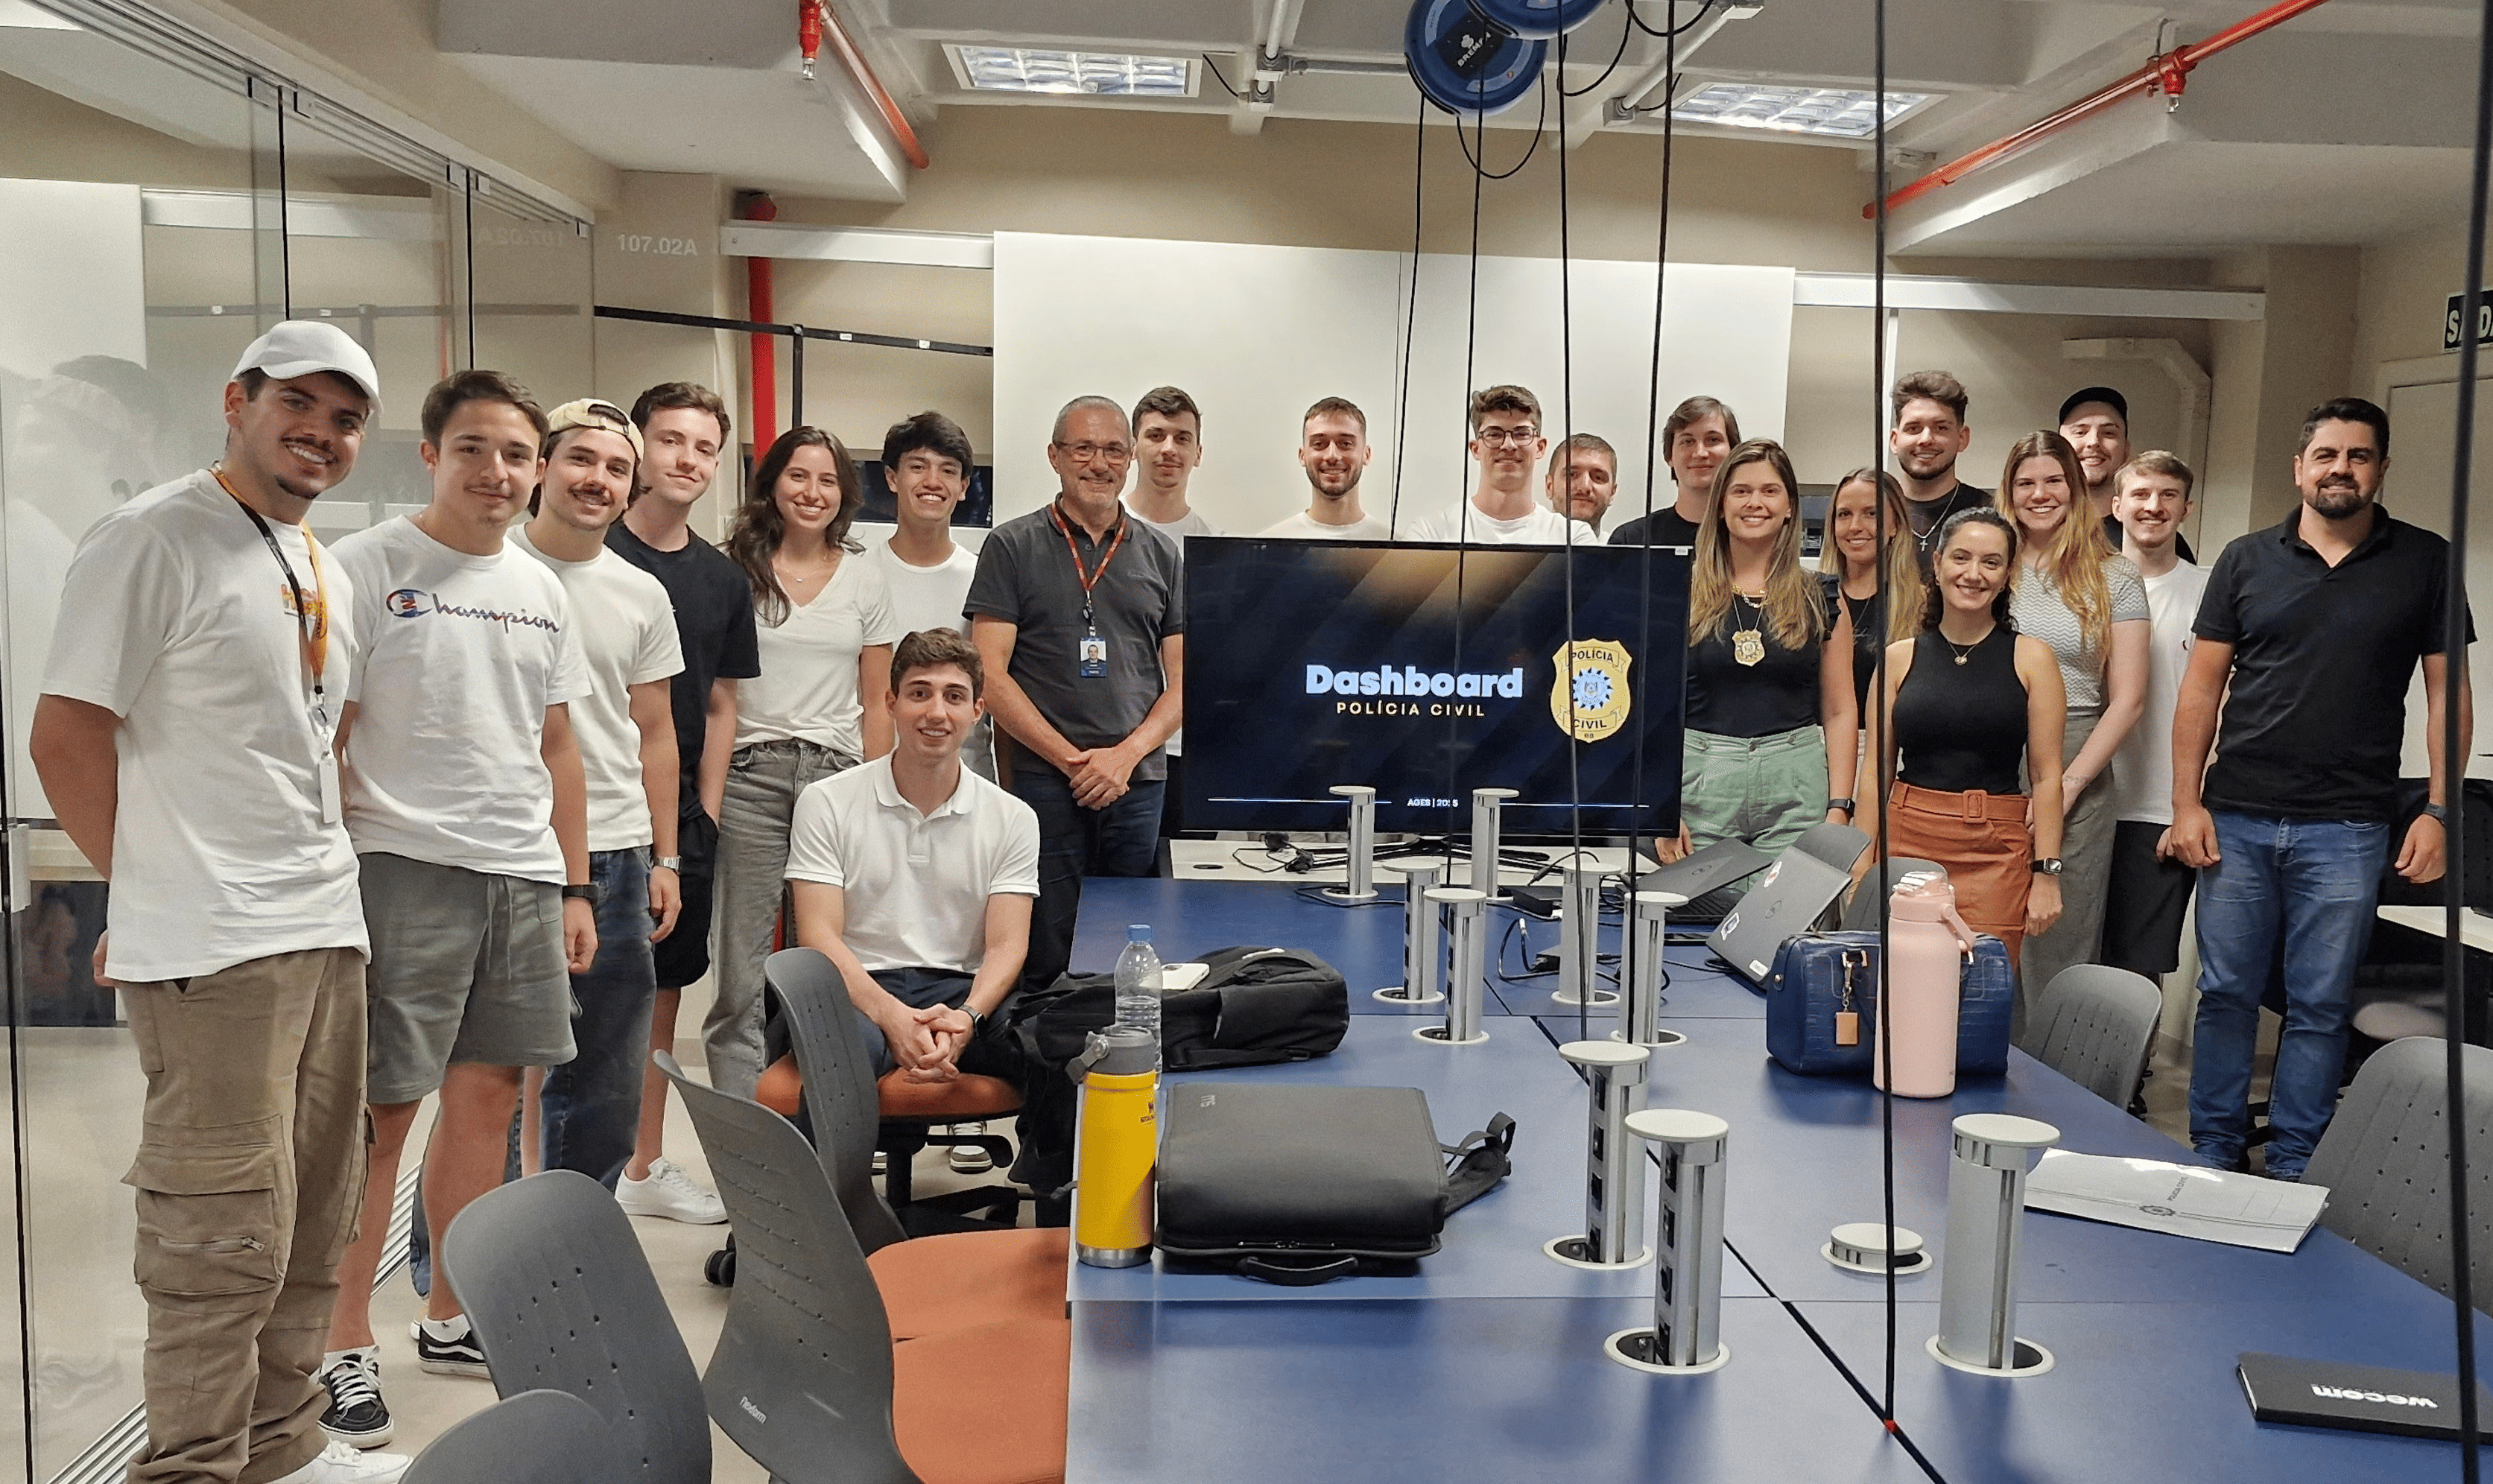
\includegraphics[width=1\linewidth]{conteudo/3 - ages II/conteudo/figures/equipe-policia-civil.png}
    \textit{Fonte: Wiki do Projeto}
    \label{fig:projeto-time}
\end{figure}
\section[Desenvolvimento do Projeto]{Desenvolvimento do Projeto}



\subsection*{Repositório do Código Fonte do Projeto}
    Um repositório público foi estabelecido no GitLab da AGES, abrangendo sete componentes distintos: api-auth, api-medico, infraestrutura, web-administrador, web- médico, web-site e uma seção dedicada à documentação no formato de Wiki.

    Para mais detalhes, consulte este link:
    {\url{https://tools.ages.pucrs.br/let-me-trial}}.


\subsection{Banco de Dados Utilizado}
  O banco de dados escolhido para o projeto foi do tipo relacional. Utilizamos PostgreSQL devido aos recursos avançados, como transações ACID (Atomicidade, Consistência, Isolamento e Durabilidade). Na \texttt{\href{http://example.com}{wiki}} do repositório, há uma seção dedicada ao banco de dados (BD), onde está detalhada toda a estrutura utilizada no projeto. Você pode visualizar o modelo conceitual completo do banco de dados na figura abaixo.


\subsection{Arquitetura Utilizada}
  Como arquitetura para o projeto, foi escolhida a arquitetura hexagonal. A arquitetura hexagonal, também conhecida como arquitetura ports and adapters, é um padrão de arquitetura de software que promove a separação clara entre a lógica de negócios e os detalhes de implementação técnica. Ela facilita a modularidade, testabilidade e manutenção do sistema, ao permitir a substituição fácil de componentes externos e a reutilização de lógicas de negócio em diferentes contextos.\\
    Na wiki do repositório, há uma seção dedicada à Arquitetura que detalha a estrutura completa. Um diagrama de alto nível ilustrando essa arquitetura pode ser encontrado na figura abaixo.


\subsection{Protótipos das Telas Desenvolvidas}
  Deverão ser apresentados os links da Wiki, com uma breve descrição.

\subsection{Tecnologias Utilizadas}
  Para o desenvolvimento do frontend, utilizamos as seguintes tecnologias principais:\\
React: Uma biblioteca JavaScript amplamente usada para construir interfaces de usuário dinâmicas e responsivas.\\
Next.js: Um framework sobre React que suporta renderização no lado do servidor (SSR) e otimização de desempenho, ideal para aplicações web escaláveis.\\
JavaScript/TypeScript: Linguagens de programação essenciais para implementar a lógica da aplicação, com TypeScript oferecendo tipagem estática opcional para um desenvolvimento mais robusto e seguro.\\

Além disso, utilizamos as seguintes bibliotecas e ferramentas específicas:
Axios: Uma biblioteca para realizar requisições HTTP de forma simplificada e eficiente.\\

Keycloak: Um sistema de gerenciamento de identidade e acesso utilizado para autenticação e autorização seguras.\\
React Router (quando necessário em Next.js): Uma biblioteca para roteamento que facilita a navegação dentro de aplicações React complexas.\\

No backend, utilizamos as seguintes tecnologias:\\
Java: Uma linguagem de programação robusta e amplamente adotada para o desenvolvimento de aplicações empresariais.\\
Framework Spring Boot: Um framework Java que simplifica a criação de aplicações web e serviços RESTful, oferecendo uma configuração mínima e produtividade elevada.\\
Gerenciador de dependências Maven: Utilizado para gerenciar as dependências do projeto Java de forma eficiente e automatizada.\\
Testes com JUnit: Um framework de testes unitários para Java que facilita a implementação e execução de testes automatizados.\\

Ao acessar a wiki dentro do repositório, é possível encontrar a seção Frontend e Backend, onde é detalhada toda as tecnologias utilizadas no projeto.

\section[Atividades Desempenhadas Pelo Aluno no Projeto]{Atividades Desempenhadas Pelo Aluno no Projeto}

\subsection{Sprint 0}

No mínimo uma página contendo tudo que o aluno fez na Sprint 0.
O projeto "Dashboard para a Polícia Civil" teve início com a Sprint 0, onde a equipe se reuniu para alinhar a visão geral do projeto e definir as diretrizes para as atividades subsequentes. A primeira tarefa da Sprint foi a criação dos protótipos no Figma e a modelagem do Banco de Dados utilizando o Astah, ferramentas essenciais para o desenvolvimento inicial do projeto. Durante a Sprint, a equipe trabalhou para definir as interfaces de usuário e a estrutura de dados, garantindo que as necessidades da Polícia Civil fossem atendidas de forma eficiente.\\
Como AGES II, fiquei encarregado da modelagem do banco de dados, em colaboração com os outros AGES II. Juntos, trabalhamos na definição das tabelas e seus relacionamentos no Astah, o que ajudou a garantir que a estrutura de dados fosse eficiente e escalável para o uso no dashboard. Além disso, devido à minha experiência na modelagem do banco de dados, pude contribuir com minha experiência para a criação de algumas telas no Figma, focadas nos gráficos de dashboards. Essas telas foram projetadas com base nas planilhas que seriam integradas ao sistema, o que me proporcionou um entendimento mais profundo sobre quais tipos de gráficos seriam mais apropriados para a aplicação e como visualizá-los de forma clara e eficiente.\\
Durante a execução dessa Sprint, não foram encontrados problemas significativos. As atividades previstas foram completadas dentro do prazo, sem obstáculos ou dificuldades técnicas. A equipe conseguiu cumprir todos os objetivos propostos, refletindo um bom alinhamento entre os membros, o que reflete uma boa organização e alinhamento entre os membros.

\subsection{Sprint 1}

Após a apresentação dos resultados da Sprint 0 aos stakeholders, onde mostramos os fluxogramas e mockups desenvolvidos, e onde discutimos o planejamento para a Sprint 1, nossa equipe foi organizada em quatro squads. Cada squad foi composta por uma divisão equilibrada entre membros focados em backend e frontend. Eu fui alocado na squad 4, que recebeu a responsabilidade pela User Story 03, dedicada ao cadastro de pacientes.\\

Essa user story especificamente envolvia o desenvolvimento de funcionalidades para cadastrar pacientes sob a supervisão de um médico. Como ainda não havíamos implementado a funcionalidade de cadastro de médicos, utilizamos um médico de teste para integrar essa nova funcionalidade. Junto com Guilherme Ochoa, também do backend da squad 4, decidimos adotar uma abordagem colaborativa em vez de dividir tarefas especificamente. Optamos por trabalhar juntos em todos os aspectos da funcionalidade, o que nos permitiu aprender e complementar um ao outro de maneira mais eficiente.\\

Inicialmente, enfrentei desafios significativos devido à falta de experiência prática com projetos reais. Foi durante esse período que foi percebido a importância do Pair Programming, uma técnica de programação colaborativa que se provou fundamental para o meu desenvolvimento. Nas sessões de Pair Programming, realizadas virtualmente, recebi orientação intensiva do AGES IV sobre a arquitetura hexagonal utilizada no backend. Essa orientação foi crucial para entender onde e como implementar cada segmento da funcionalidade em desenvolvimento.\\

Focamos inicialmente na criação de funções robustas para a verificação de dados e tratamento de exceções. Após estabelecermos uma base sólida para a funcionalidade de cadastro, prosseguimos para a etapa de testes.\\

Em colaboração com o AGES IV, desenvolvemos testes unitários utilizando a biblioteca Mockito. A experiência de desenvolver testes unitários foi enriquecedora, proporcionando uma compreensão mais profunda das práticas de desenvolvimento de software e da importância de uma base de código testável e sustentável.\\

A Sprint 1 provou ser uma experiência intensiva e instrutiva, consolidando as habilidades técnicas da equipe e aprimorando nossa capacidade de trabalhar de forma colaborativa sob a estrutura de desenvolvimento ágil. As lições aprendidas e as habilidades desenvolvidas durante essa fase do projeto serão fundamentais para o sucesso das próximas sprints.
O projeto "Dashboard para a Polícia Civil" avançou para a Sprint 1, onde a equipe foi dividida em duas áreas de atuação: frontend e backend. Cada membro foi designado para sua respectiva área, e como eu fui designado para o backend, a minha principal tarefa na Sprint 1 foi a criação de uma rota para receber arquivos CSV, além de realizar alterações no banco de dados conforme a necessidade para atender aos requisitos do sistema. A equipe estava focada na integração de dados externos através de arquivos CSV, o que exigia uma lógica robusta para garantir a integridade e a consistência desses dados dentro da aplicação.\\
Durante a Sprint 1, consegui concluir a criação da rota para receber arquivos CSV, bem como implementar a lógica para ler o arquivo e validá-lo de forma eficiente. Uma parte importante desse processo foi a implementação da lógica para direcionar cada tipo de arquivo para a função responsável por sua validação. Para garantir que o código fosse flexível e fácil de expandir no futuro, utilizei o design pattern 'strategy'. Com esse padrão, a lógica foi modularizada, permitindo que novos tipos de validação fossem facilmente adicionados sem a necessidade de modificar o código existente.\\
Além dessas atividades, também comecei a implementação de uma possível pipeline para o projeto de backend-file, com foco na automação de processos de integração contínua e entrega contínua (CI/CD) utilizando GitLab. Embora essa implementação ainda esteja em seus estágios iniciais, ela representa um avanço importante para garantir a escalabilidade e a manutenção do projeto.\\
Durante a execução da Sprint 1, enfrentei alguns problemas para rodar a aplicação de infraestrutura no meu computador pelo Docker, o que causou algum atraso no início das atividades. No entanto, esse problema não afetou significativamente minha capacidade de concluir as tarefas previstas, e com a ajuda dos colegas, consegui superar esse obstáculo rapidamente.

\subsection{Sprint 2}

No mínimo uma página contendo tudo que o aluno fez na Sprint 2.
\subsection{Sprint 3}
No mínimo uma página contendo tudo que o aluno fez na Sprint 3.
\subsection{Sprint 4}

No mínimo uma página contendo tudo que o aluno fez na Sprint 4.
\section[Conclusão]{Conclusão}

Participar da minha primeira AGES tem sido um desafio significativo, especialmente em acompanhar o ritmo do projeto devido à minha falta de autonomia nas tarefas designadas. Grande parte do tempo, minha participação tem sido predominantemente em pair programming. Essa metodologia tem se mostrado extremamente benéfica, não apenas pela aprendizagem técnica, mas também pelo suporte contínuo que recebo do AGES IV. Ele tem se destacado por sua disposição em explicar detalhadamente os processos e solucionar quaisquer dúvidas que surgem, o que tem sido crucial para o meu desenvolvimento no projeto.\\
O pair programming tem reforçado minhas habilidades técnicas — as hardskills
— consideravelmente. A troca constante de informações e a colaboração direta com colegas mais experientes têm acelerado meu aprendizado, proporcionando um entendimento mais profundo das tecnologias e técnicas utilizadas. Essa experiência tem mostrado o valor da comunicação efetiva, uma habilidade que possuo e e que tem sido essencial para expressar minhas dificuldades e solicitar ajuda sempre que necessário.\\
Além disso, os conhecimentos adquiridos em disciplinas anteriores do curso, como Gerenciamento e Configuração de Software, Algoritmos e Estruturas de Dados, e principalmente Programação Orientada a Objetos, têm se mostrado fundamentais. Essas disciplinas forneceram uma base sólida que agora aplico no contexto prático do projeto, facilitando a compreensão e implementação das demandas técnicas.\\
A experiência geral neste projeto inicial tem sido extremamente positiva. Os dois líderes da AGES IV demonstram competência e compromisso, sempre prontos para apoiar o restante da equipe. Eles têm desempenhado um papel crucial, especialmente na arquitetura do projeto, uma área que apresentou desafios significativos devido à ausência dos membros da AGES III nas primeiras sprints. A liderança eficaz e o ambiente colaborativo têm não só mitigado esses desafios, mas também enriquecido a minha experiência de aprendizado.\\

Este primeiro contato com a AGES está provando ser uma introdução valiosa ao mundo do desenvolvimento de software em um ambiente ágil e suportado, preparando-me não apenas para as demandas futuras deste projeto, mas também para outras iniciativas profissionais.

  \chapter[AGES I --- “LET ME TRIAL 2024/1”]{AGES I --- “LET ME TRIAL 2024/1”}

\section[Introdução]{Introdução}

O projeto de desenvolvimento do dashboard para a Polícia Civil foi realizado durante o semestre de 2025/1, com reuniões regulares nas terças-feiras e quintas-feiras, das 17h30 às 19h00, com o objetivo de atender à necessidade de centralizar e analisar dados operacionais e administrativos de maneira eficiente. Este projeto visa criar uma solução para a visualização de dados em tempo real, permitindo uma gestão mais ágil e eficaz para os gestores da Polícia Civil, como o Chefe de Polícia e os Diretores de Departamentos. \\
A proposta surge da necessidade de integrar dados de diferentes departamentos, divisões e delegacias da Polícia Civil, oferecendo uma visão abrangente das operações e desempenho dos agentes. Atualmente, há uma dificuldade na visualização e interpretação desses dados, impactando a rapidez nas tomadas de decisão. Com a criação deste dashboard, será possível analisar indicadores como produtividade, número de ocorrências, tempo de resolução e desempenho dos agentes, melhorando a eficácia das ações e intervenções da polícia. \\
O sistema será acessível por navegadores web e dispositivos móveis, oferecendo flexibilidade e mobilidade aos gestores. O dashboard terá funcionalidades como visualizações gráficas dinâmicas, filtros personalizados e alertas em tempo real, proporcionando uma ferramenta essencial para a gestão estratégica e operacional da Polícia Civil. \\
O projeto será conduzido de acordo com a metodologia ágil, com encontros periódicos com os stakeholders, para garantir alinhamento contínuo entre as expectativas do cliente e os resultados alcançados. A seguir, a duração detalhada de cada Sprint será apresentada, ilustrando o planejamento do trabalho e os marcos atingidos ao longo do projeto.

\begin{table}[H]
    \centering
    \caption{Período de cada Sprint - AGES II}
    \begin{tabular}{|c|c|}
        \hline
        \textbf{Sprints} & \textbf{Período} \\
        \hline
        0 & 08/03/2024 a 22/03/2024\\
        1 & 22/03/2024 a 19/04/2024 \\
        2 & 119/04/2024 a 10/05/2024 \\
        3 & 10/05/2024 a 31/05/2024 \\
        4 & 31/05/2024 a 21/06/2024 \\
        \hline
    \end{tabular}
\end{table}

Este projeto foi desenvolvido sob a orientação do professor Dilnei Venturini. A equipe responsável pelo projeto ’Dashboard para a Polícia Civil’ está retratada na Figura 2.


\begin{figure}[H]
    \centering
    \small
    \caption{Time responsável pelo projeto}
    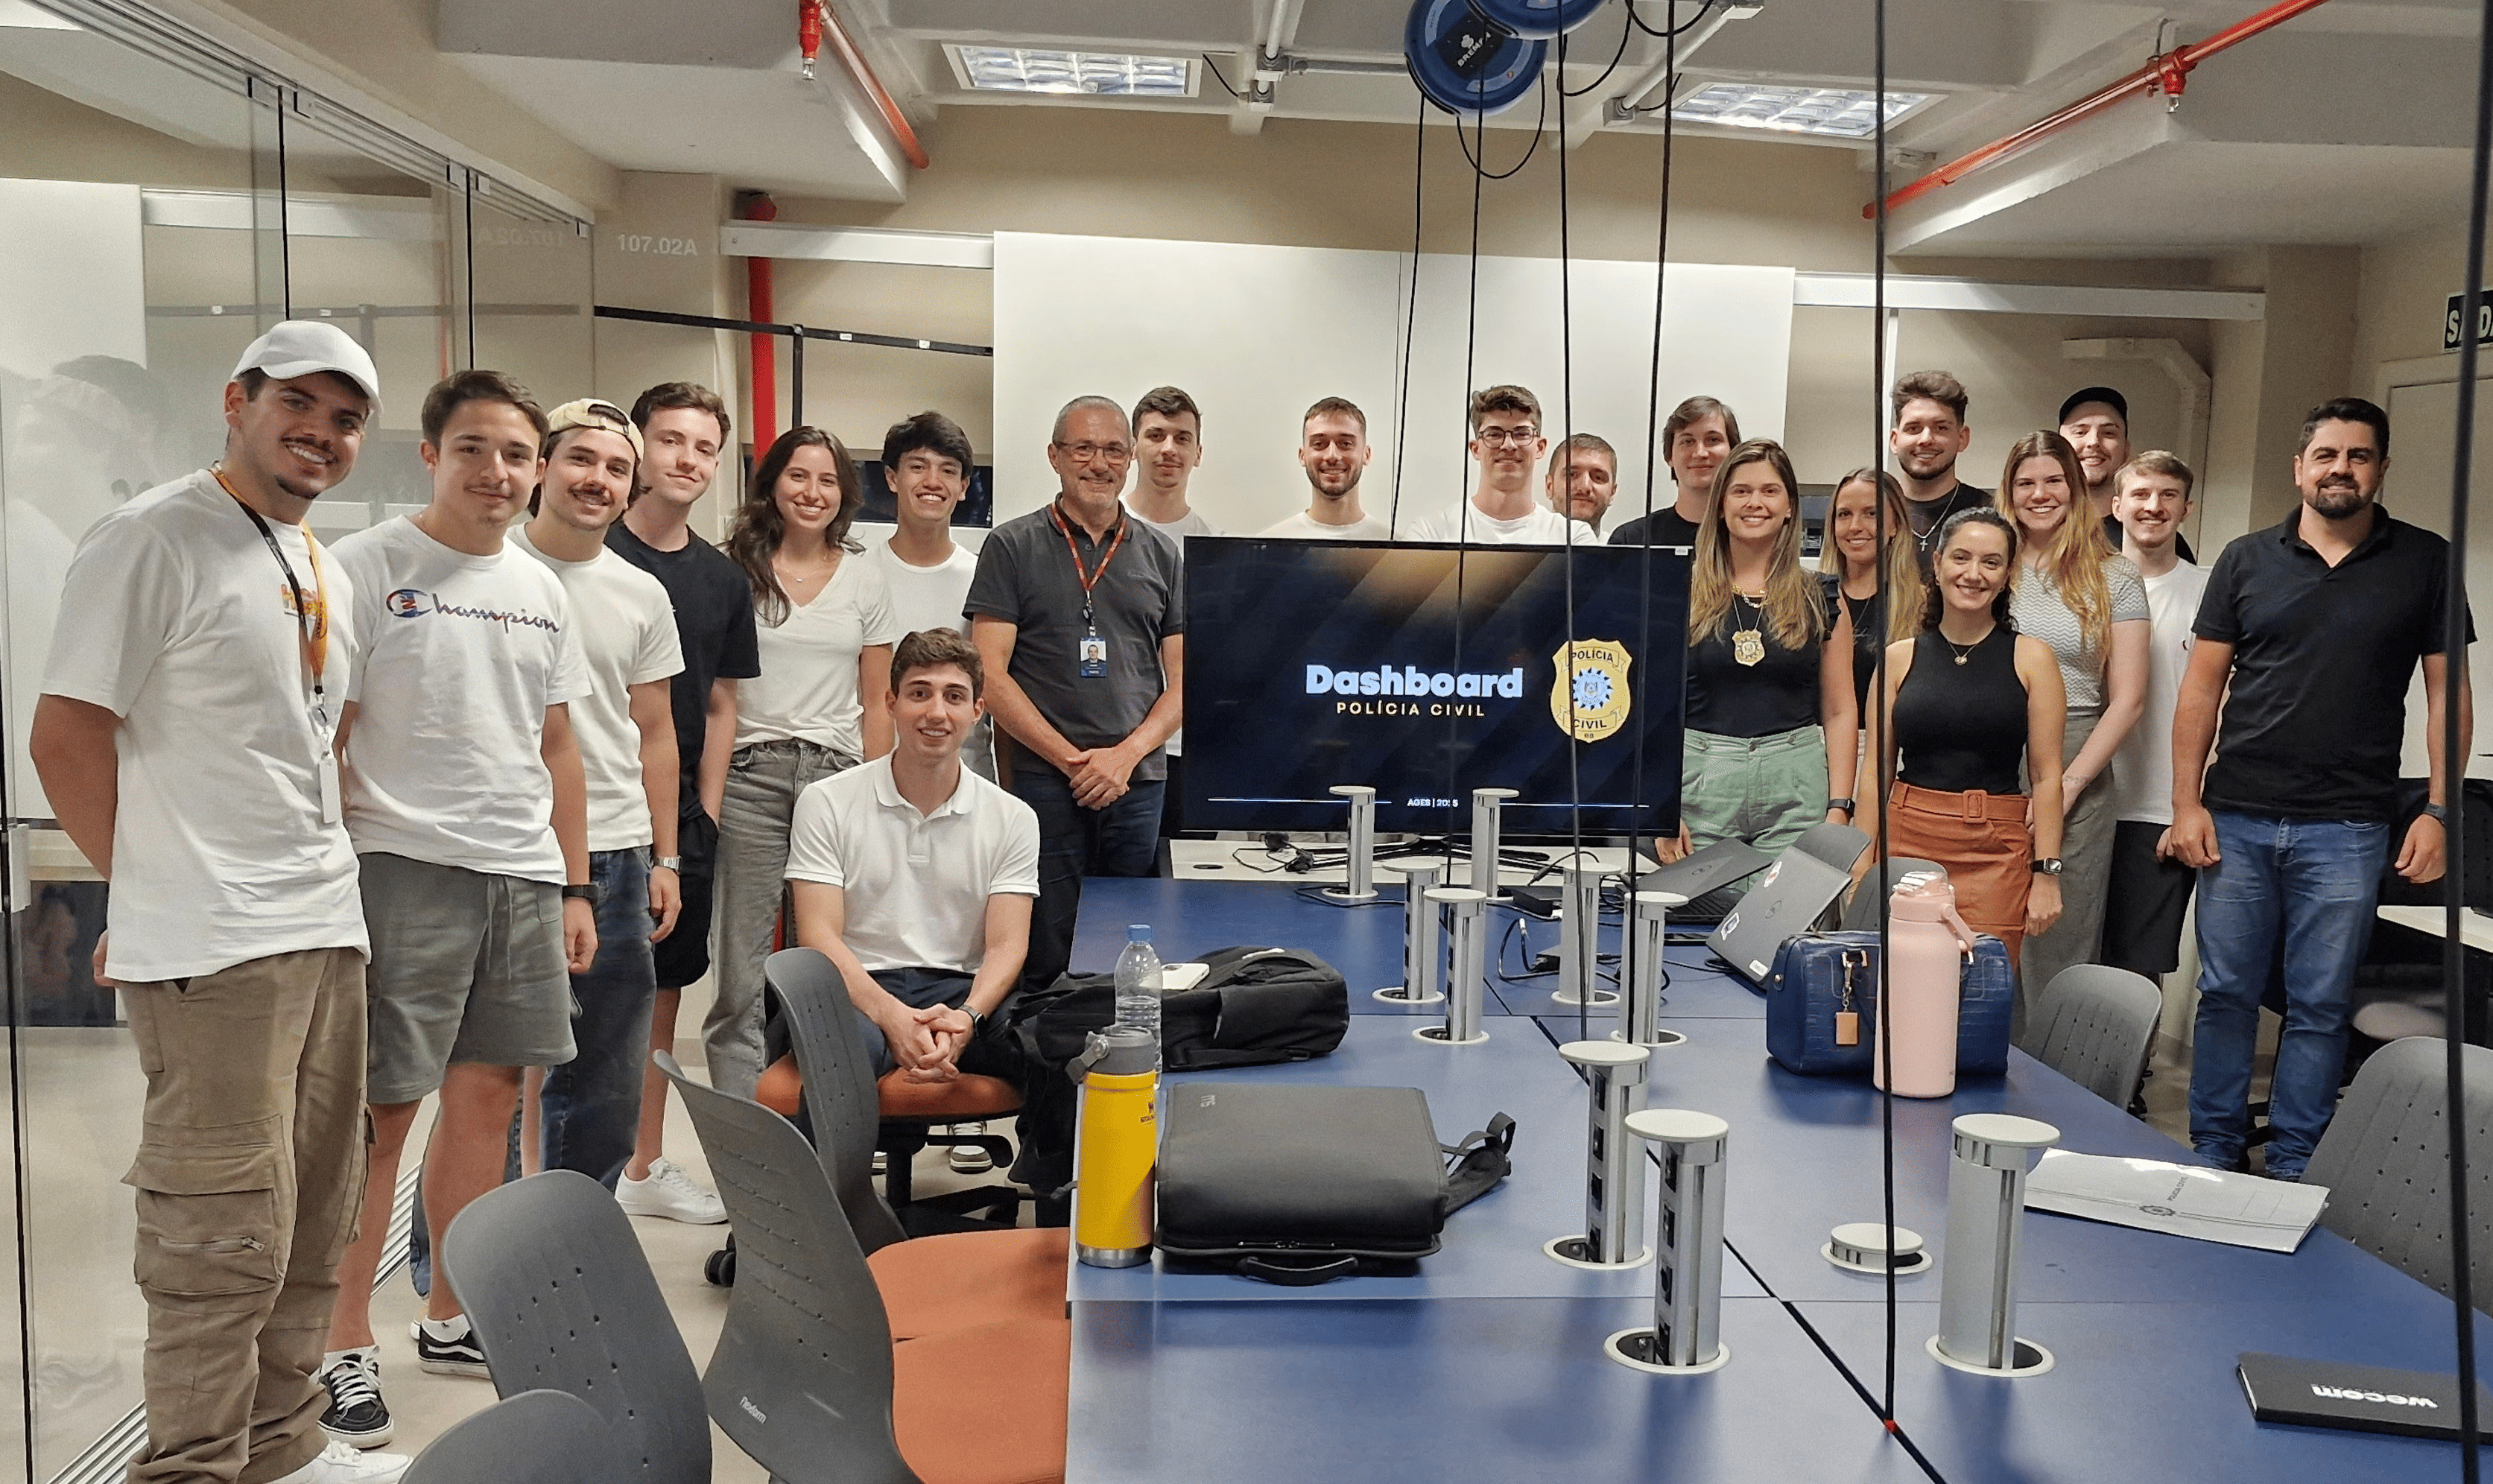
\includegraphics[width=1\linewidth]{conteudo/3 - ages II/conteudo/figures/equipe-policia-civil.png}
    \textit{Fonte: Wiki do Projeto}
    \label{fig:projeto-time}
\end{figure}
\section[Desenvolvimento do Projeto]{Desenvolvimento do Projeto}



\subsection*{Repositório do Código Fonte do Projeto}
    Um repositório público foi estabelecido no GitLab da AGES, abrangendo sete componentes distintos: api-auth, api-medico, infraestrutura, web-administrador, web- médico, web-site e uma seção dedicada à documentação no formato de Wiki.

    Para mais detalhes, consulte este link:
    {\url{https://tools.ages.pucrs.br/let-me-trial}}.


\subsection{Banco de Dados Utilizado}
  O banco de dados escolhido para o projeto foi do tipo relacional. Utilizamos PostgreSQL devido aos recursos avançados, como transações ACID (Atomicidade, Consistência, Isolamento e Durabilidade). Na \texttt{\href{http://example.com}{wiki}} do repositório, há uma seção dedicada ao banco de dados (BD), onde está detalhada toda a estrutura utilizada no projeto. Você pode visualizar o modelo conceitual completo do banco de dados na figura abaixo.


\subsection{Arquitetura Utilizada}
  Como arquitetura para o projeto, foi escolhida a arquitetura hexagonal. A arquitetura hexagonal, também conhecida como arquitetura ports and adapters, é um padrão de arquitetura de software que promove a separação clara entre a lógica de negócios e os detalhes de implementação técnica. Ela facilita a modularidade, testabilidade e manutenção do sistema, ao permitir a substituição fácil de componentes externos e a reutilização de lógicas de negócio em diferentes contextos.\\
    Na wiki do repositório, há uma seção dedicada à Arquitetura que detalha a estrutura completa. Um diagrama de alto nível ilustrando essa arquitetura pode ser encontrado na figura abaixo.


\subsection{Protótipos das Telas Desenvolvidas}
  Deverão ser apresentados os links da Wiki, com uma breve descrição.

\subsection{Tecnologias Utilizadas}
  Para o desenvolvimento do frontend, utilizamos as seguintes tecnologias principais:\\
React: Uma biblioteca JavaScript amplamente usada para construir interfaces de usuário dinâmicas e responsivas.\\
Next.js: Um framework sobre React que suporta renderização no lado do servidor (SSR) e otimização de desempenho, ideal para aplicações web escaláveis.\\
JavaScript/TypeScript: Linguagens de programação essenciais para implementar a lógica da aplicação, com TypeScript oferecendo tipagem estática opcional para um desenvolvimento mais robusto e seguro.\\

Além disso, utilizamos as seguintes bibliotecas e ferramentas específicas:
Axios: Uma biblioteca para realizar requisições HTTP de forma simplificada e eficiente.\\

Keycloak: Um sistema de gerenciamento de identidade e acesso utilizado para autenticação e autorização seguras.\\
React Router (quando necessário em Next.js): Uma biblioteca para roteamento que facilita a navegação dentro de aplicações React complexas.\\

No backend, utilizamos as seguintes tecnologias:\\
Java: Uma linguagem de programação robusta e amplamente adotada para o desenvolvimento de aplicações empresariais.\\
Framework Spring Boot: Um framework Java que simplifica a criação de aplicações web e serviços RESTful, oferecendo uma configuração mínima e produtividade elevada.\\
Gerenciador de dependências Maven: Utilizado para gerenciar as dependências do projeto Java de forma eficiente e automatizada.\\
Testes com JUnit: Um framework de testes unitários para Java que facilita a implementação e execução de testes automatizados.\\

Ao acessar a wiki dentro do repositório, é possível encontrar a seção Frontend e Backend, onde é detalhada toda as tecnologias utilizadas no projeto.

\section[Atividades Desempenhadas Pelo Aluno no Projeto]{Atividades Desempenhadas Pelo Aluno no Projeto}

\subsection{Sprint 0}

No mínimo uma página contendo tudo que o aluno fez na Sprint 0.
O projeto "Dashboard para a Polícia Civil" teve início com a Sprint 0, onde a equipe se reuniu para alinhar a visão geral do projeto e definir as diretrizes para as atividades subsequentes. A primeira tarefa da Sprint foi a criação dos protótipos no Figma e a modelagem do Banco de Dados utilizando o Astah, ferramentas essenciais para o desenvolvimento inicial do projeto. Durante a Sprint, a equipe trabalhou para definir as interfaces de usuário e a estrutura de dados, garantindo que as necessidades da Polícia Civil fossem atendidas de forma eficiente.\\
Como AGES II, fiquei encarregado da modelagem do banco de dados, em colaboração com os outros AGES II. Juntos, trabalhamos na definição das tabelas e seus relacionamentos no Astah, o que ajudou a garantir que a estrutura de dados fosse eficiente e escalável para o uso no dashboard. Além disso, devido à minha experiência na modelagem do banco de dados, pude contribuir com minha experiência para a criação de algumas telas no Figma, focadas nos gráficos de dashboards. Essas telas foram projetadas com base nas planilhas que seriam integradas ao sistema, o que me proporcionou um entendimento mais profundo sobre quais tipos de gráficos seriam mais apropriados para a aplicação e como visualizá-los de forma clara e eficiente.\\
Durante a execução dessa Sprint, não foram encontrados problemas significativos. As atividades previstas foram completadas dentro do prazo, sem obstáculos ou dificuldades técnicas. A equipe conseguiu cumprir todos os objetivos propostos, refletindo um bom alinhamento entre os membros, o que reflete uma boa organização e alinhamento entre os membros.

\subsection{Sprint 1}

Após a apresentação dos resultados da Sprint 0 aos stakeholders, onde mostramos os fluxogramas e mockups desenvolvidos, e onde discutimos o planejamento para a Sprint 1, nossa equipe foi organizada em quatro squads. Cada squad foi composta por uma divisão equilibrada entre membros focados em backend e frontend. Eu fui alocado na squad 4, que recebeu a responsabilidade pela User Story 03, dedicada ao cadastro de pacientes.\\

Essa user story especificamente envolvia o desenvolvimento de funcionalidades para cadastrar pacientes sob a supervisão de um médico. Como ainda não havíamos implementado a funcionalidade de cadastro de médicos, utilizamos um médico de teste para integrar essa nova funcionalidade. Junto com Guilherme Ochoa, também do backend da squad 4, decidimos adotar uma abordagem colaborativa em vez de dividir tarefas especificamente. Optamos por trabalhar juntos em todos os aspectos da funcionalidade, o que nos permitiu aprender e complementar um ao outro de maneira mais eficiente.\\

Inicialmente, enfrentei desafios significativos devido à falta de experiência prática com projetos reais. Foi durante esse período que foi percebido a importância do Pair Programming, uma técnica de programação colaborativa que se provou fundamental para o meu desenvolvimento. Nas sessões de Pair Programming, realizadas virtualmente, recebi orientação intensiva do AGES IV sobre a arquitetura hexagonal utilizada no backend. Essa orientação foi crucial para entender onde e como implementar cada segmento da funcionalidade em desenvolvimento.\\

Focamos inicialmente na criação de funções robustas para a verificação de dados e tratamento de exceções. Após estabelecermos uma base sólida para a funcionalidade de cadastro, prosseguimos para a etapa de testes.\\

Em colaboração com o AGES IV, desenvolvemos testes unitários utilizando a biblioteca Mockito. A experiência de desenvolver testes unitários foi enriquecedora, proporcionando uma compreensão mais profunda das práticas de desenvolvimento de software e da importância de uma base de código testável e sustentável.\\

A Sprint 1 provou ser uma experiência intensiva e instrutiva, consolidando as habilidades técnicas da equipe e aprimorando nossa capacidade de trabalhar de forma colaborativa sob a estrutura de desenvolvimento ágil. As lições aprendidas e as habilidades desenvolvidas durante essa fase do projeto serão fundamentais para o sucesso das próximas sprints.
O projeto "Dashboard para a Polícia Civil" avançou para a Sprint 1, onde a equipe foi dividida em duas áreas de atuação: frontend e backend. Cada membro foi designado para sua respectiva área, e como eu fui designado para o backend, a minha principal tarefa na Sprint 1 foi a criação de uma rota para receber arquivos CSV, além de realizar alterações no banco de dados conforme a necessidade para atender aos requisitos do sistema. A equipe estava focada na integração de dados externos através de arquivos CSV, o que exigia uma lógica robusta para garantir a integridade e a consistência desses dados dentro da aplicação.\\
Durante a Sprint 1, consegui concluir a criação da rota para receber arquivos CSV, bem como implementar a lógica para ler o arquivo e validá-lo de forma eficiente. Uma parte importante desse processo foi a implementação da lógica para direcionar cada tipo de arquivo para a função responsável por sua validação. Para garantir que o código fosse flexível e fácil de expandir no futuro, utilizei o design pattern 'strategy'. Com esse padrão, a lógica foi modularizada, permitindo que novos tipos de validação fossem facilmente adicionados sem a necessidade de modificar o código existente.\\
Além dessas atividades, também comecei a implementação de uma possível pipeline para o projeto de backend-file, com foco na automação de processos de integração contínua e entrega contínua (CI/CD) utilizando GitLab. Embora essa implementação ainda esteja em seus estágios iniciais, ela representa um avanço importante para garantir a escalabilidade e a manutenção do projeto.\\
Durante a execução da Sprint 1, enfrentei alguns problemas para rodar a aplicação de infraestrutura no meu computador pelo Docker, o que causou algum atraso no início das atividades. No entanto, esse problema não afetou significativamente minha capacidade de concluir as tarefas previstas, e com a ajuda dos colegas, consegui superar esse obstáculo rapidamente.

\subsection{Sprint 2}

No mínimo uma página contendo tudo que o aluno fez na Sprint 2.
\subsection{Sprint 3}
No mínimo uma página contendo tudo que o aluno fez na Sprint 3.
\subsection{Sprint 4}

No mínimo uma página contendo tudo que o aluno fez na Sprint 4.
\section[Conclusão]{Conclusão}

Participar da minha primeira AGES tem sido um desafio significativo, especialmente em acompanhar o ritmo do projeto devido à minha falta de autonomia nas tarefas designadas. Grande parte do tempo, minha participação tem sido predominantemente em pair programming. Essa metodologia tem se mostrado extremamente benéfica, não apenas pela aprendizagem técnica, mas também pelo suporte contínuo que recebo do AGES IV. Ele tem se destacado por sua disposição em explicar detalhadamente os processos e solucionar quaisquer dúvidas que surgem, o que tem sido crucial para o meu desenvolvimento no projeto.\\
O pair programming tem reforçado minhas habilidades técnicas — as hardskills
— consideravelmente. A troca constante de informações e a colaboração direta com colegas mais experientes têm acelerado meu aprendizado, proporcionando um entendimento mais profundo das tecnologias e técnicas utilizadas. Essa experiência tem mostrado o valor da comunicação efetiva, uma habilidade que possuo e e que tem sido essencial para expressar minhas dificuldades e solicitar ajuda sempre que necessário.\\
Além disso, os conhecimentos adquiridos em disciplinas anteriores do curso, como Gerenciamento e Configuração de Software, Algoritmos e Estruturas de Dados, e principalmente Programação Orientada a Objetos, têm se mostrado fundamentais. Essas disciplinas forneceram uma base sólida que agora aplico no contexto prático do projeto, facilitando a compreensão e implementação das demandas técnicas.\\
A experiência geral neste projeto inicial tem sido extremamente positiva. Os dois líderes da AGES IV demonstram competência e compromisso, sempre prontos para apoiar o restante da equipe. Eles têm desempenhado um papel crucial, especialmente na arquitetura do projeto, uma área que apresentou desafios significativos devido à ausência dos membros da AGES III nas primeiras sprints. A liderança eficaz e o ambiente colaborativo têm não só mitigado esses desafios, mas também enriquecido a minha experiência de aprendizado.\\

Este primeiro contato com a AGES está provando ser uma introdução valiosa ao mundo do desenvolvimento de software em um ambiente ágil e suportado, preparando-me não apenas para as demandas futuras deste projeto, mas também para outras iniciativas profissionais.

  \chapter[AGES I --- “LET ME TRIAL 2024/1”]{AGES I --- “LET ME TRIAL 2024/1”}

\section[Introdução]{Introdução}

O projeto de desenvolvimento do dashboard para a Polícia Civil foi realizado durante o semestre de 2025/1, com reuniões regulares nas terças-feiras e quintas-feiras, das 17h30 às 19h00, com o objetivo de atender à necessidade de centralizar e analisar dados operacionais e administrativos de maneira eficiente. Este projeto visa criar uma solução para a visualização de dados em tempo real, permitindo uma gestão mais ágil e eficaz para os gestores da Polícia Civil, como o Chefe de Polícia e os Diretores de Departamentos. \\
A proposta surge da necessidade de integrar dados de diferentes departamentos, divisões e delegacias da Polícia Civil, oferecendo uma visão abrangente das operações e desempenho dos agentes. Atualmente, há uma dificuldade na visualização e interpretação desses dados, impactando a rapidez nas tomadas de decisão. Com a criação deste dashboard, será possível analisar indicadores como produtividade, número de ocorrências, tempo de resolução e desempenho dos agentes, melhorando a eficácia das ações e intervenções da polícia. \\
O sistema será acessível por navegadores web e dispositivos móveis, oferecendo flexibilidade e mobilidade aos gestores. O dashboard terá funcionalidades como visualizações gráficas dinâmicas, filtros personalizados e alertas em tempo real, proporcionando uma ferramenta essencial para a gestão estratégica e operacional da Polícia Civil. \\
O projeto será conduzido de acordo com a metodologia ágil, com encontros periódicos com os stakeholders, para garantir alinhamento contínuo entre as expectativas do cliente e os resultados alcançados. A seguir, a duração detalhada de cada Sprint será apresentada, ilustrando o planejamento do trabalho e os marcos atingidos ao longo do projeto.

\begin{table}[H]
    \centering
    \caption{Período de cada Sprint - AGES II}
    \begin{tabular}{|c|c|}
        \hline
        \textbf{Sprints} & \textbf{Período} \\
        \hline
        0 & 08/03/2024 a 22/03/2024\\
        1 & 22/03/2024 a 19/04/2024 \\
        2 & 119/04/2024 a 10/05/2024 \\
        3 & 10/05/2024 a 31/05/2024 \\
        4 & 31/05/2024 a 21/06/2024 \\
        \hline
    \end{tabular}
\end{table}

Este projeto foi desenvolvido sob a orientação do professor Dilnei Venturini. A equipe responsável pelo projeto ’Dashboard para a Polícia Civil’ está retratada na Figura 2.


\begin{figure}[H]
    \centering
    \small
    \caption{Time responsável pelo projeto}
    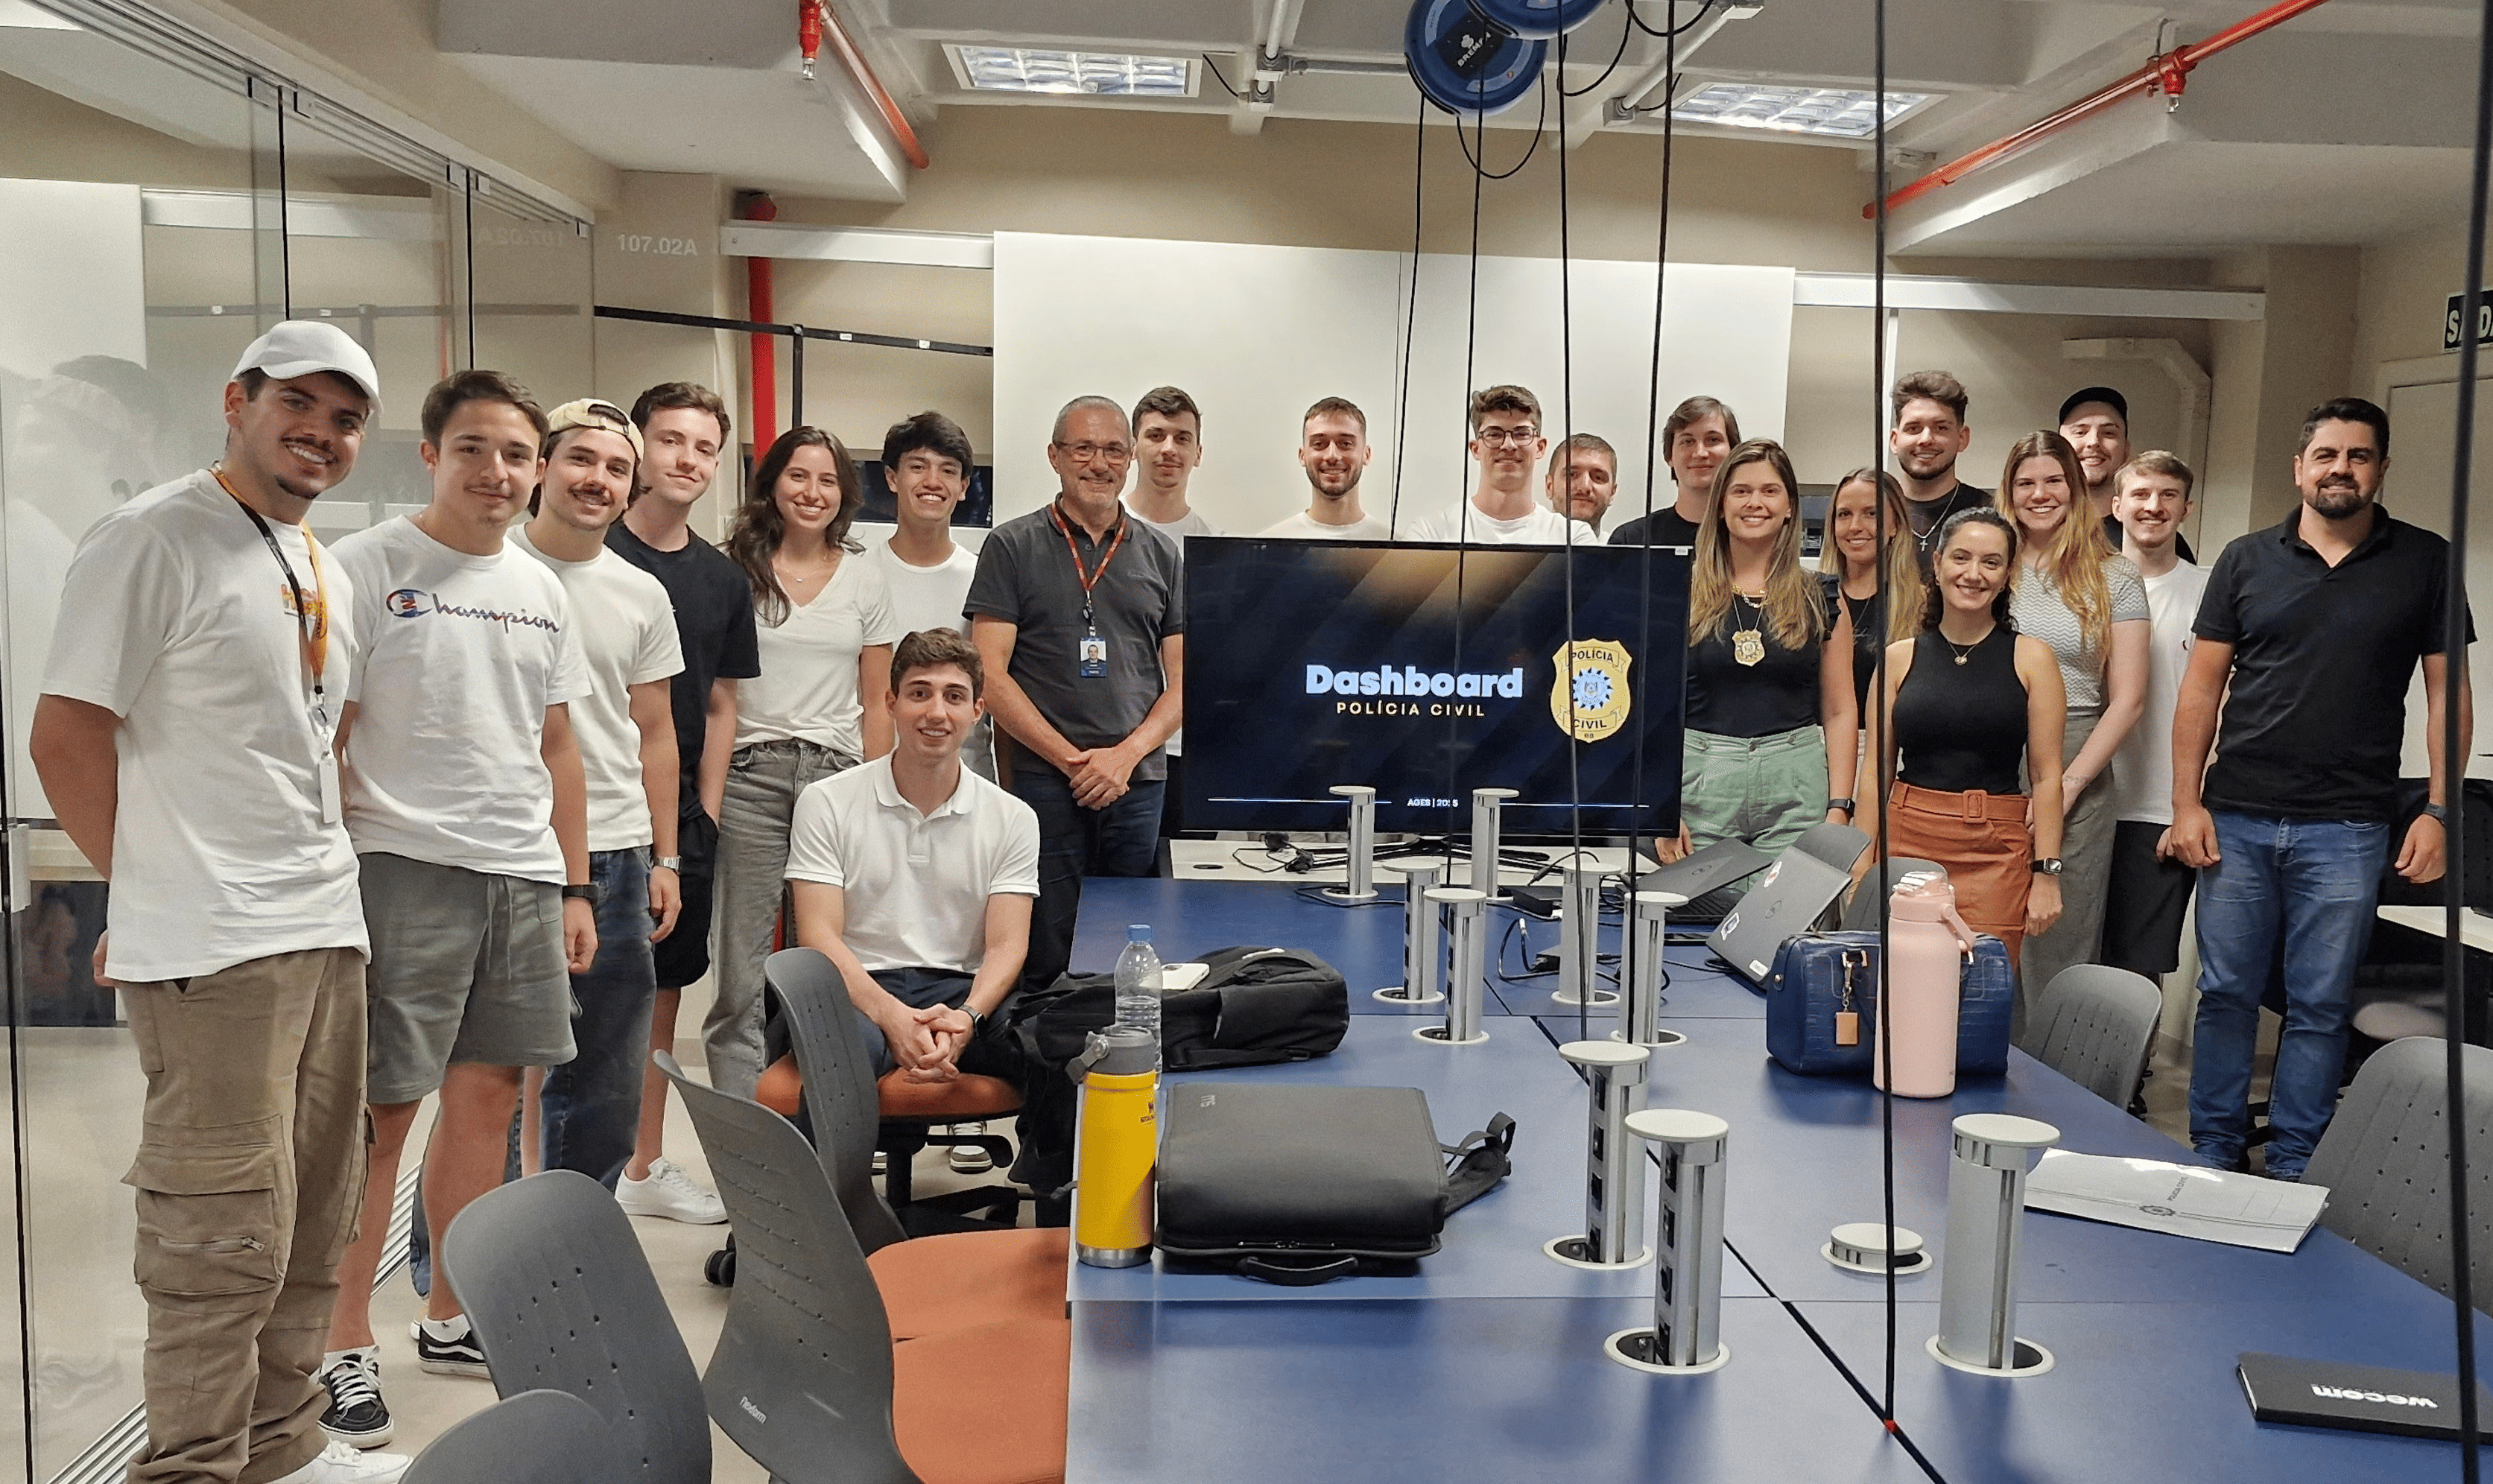
\includegraphics[width=1\linewidth]{conteudo/3 - ages II/conteudo/figures/equipe-policia-civil.png}
    \textit{Fonte: Wiki do Projeto}
    \label{fig:projeto-time}
\end{figure}
\section[Desenvolvimento do Projeto]{Desenvolvimento do Projeto}



\subsection*{Repositório do Código Fonte do Projeto}
    Um repositório público foi estabelecido no GitLab da AGES, abrangendo sete componentes distintos: api-auth, api-medico, infraestrutura, web-administrador, web- médico, web-site e uma seção dedicada à documentação no formato de Wiki.

    Para mais detalhes, consulte este link:
    {\url{https://tools.ages.pucrs.br/let-me-trial}}.


\subsection{Banco de Dados Utilizado}
  O banco de dados escolhido para o projeto foi do tipo relacional. Utilizamos PostgreSQL devido aos recursos avançados, como transações ACID (Atomicidade, Consistência, Isolamento e Durabilidade). Na \texttt{\href{http://example.com}{wiki}} do repositório, há uma seção dedicada ao banco de dados (BD), onde está detalhada toda a estrutura utilizada no projeto. Você pode visualizar o modelo conceitual completo do banco de dados na figura abaixo.


\subsection{Arquitetura Utilizada}
  Como arquitetura para o projeto, foi escolhida a arquitetura hexagonal. A arquitetura hexagonal, também conhecida como arquitetura ports and adapters, é um padrão de arquitetura de software que promove a separação clara entre a lógica de negócios e os detalhes de implementação técnica. Ela facilita a modularidade, testabilidade e manutenção do sistema, ao permitir a substituição fácil de componentes externos e a reutilização de lógicas de negócio em diferentes contextos.\\
    Na wiki do repositório, há uma seção dedicada à Arquitetura que detalha a estrutura completa. Um diagrama de alto nível ilustrando essa arquitetura pode ser encontrado na figura abaixo.


\subsection{Protótipos das Telas Desenvolvidas}
  Deverão ser apresentados os links da Wiki, com uma breve descrição.

\subsection{Tecnologias Utilizadas}
  Para o desenvolvimento do frontend, utilizamos as seguintes tecnologias principais:\\
React: Uma biblioteca JavaScript amplamente usada para construir interfaces de usuário dinâmicas e responsivas.\\
Next.js: Um framework sobre React que suporta renderização no lado do servidor (SSR) e otimização de desempenho, ideal para aplicações web escaláveis.\\
JavaScript/TypeScript: Linguagens de programação essenciais para implementar a lógica da aplicação, com TypeScript oferecendo tipagem estática opcional para um desenvolvimento mais robusto e seguro.\\

Além disso, utilizamos as seguintes bibliotecas e ferramentas específicas:
Axios: Uma biblioteca para realizar requisições HTTP de forma simplificada e eficiente.\\

Keycloak: Um sistema de gerenciamento de identidade e acesso utilizado para autenticação e autorização seguras.\\
React Router (quando necessário em Next.js): Uma biblioteca para roteamento que facilita a navegação dentro de aplicações React complexas.\\

No backend, utilizamos as seguintes tecnologias:\\
Java: Uma linguagem de programação robusta e amplamente adotada para o desenvolvimento de aplicações empresariais.\\
Framework Spring Boot: Um framework Java que simplifica a criação de aplicações web e serviços RESTful, oferecendo uma configuração mínima e produtividade elevada.\\
Gerenciador de dependências Maven: Utilizado para gerenciar as dependências do projeto Java de forma eficiente e automatizada.\\
Testes com JUnit: Um framework de testes unitários para Java que facilita a implementação e execução de testes automatizados.\\

Ao acessar a wiki dentro do repositório, é possível encontrar a seção Frontend e Backend, onde é detalhada toda as tecnologias utilizadas no projeto.

\section[Atividades Desempenhadas Pelo Aluno no Projeto]{Atividades Desempenhadas Pelo Aluno no Projeto}

\subsection{Sprint 0}

No mínimo uma página contendo tudo que o aluno fez na Sprint 0.
O projeto "Dashboard para a Polícia Civil" teve início com a Sprint 0, onde a equipe se reuniu para alinhar a visão geral do projeto e definir as diretrizes para as atividades subsequentes. A primeira tarefa da Sprint foi a criação dos protótipos no Figma e a modelagem do Banco de Dados utilizando o Astah, ferramentas essenciais para o desenvolvimento inicial do projeto. Durante a Sprint, a equipe trabalhou para definir as interfaces de usuário e a estrutura de dados, garantindo que as necessidades da Polícia Civil fossem atendidas de forma eficiente.\\
Como AGES II, fiquei encarregado da modelagem do banco de dados, em colaboração com os outros AGES II. Juntos, trabalhamos na definição das tabelas e seus relacionamentos no Astah, o que ajudou a garantir que a estrutura de dados fosse eficiente e escalável para o uso no dashboard. Além disso, devido à minha experiência na modelagem do banco de dados, pude contribuir com minha experiência para a criação de algumas telas no Figma, focadas nos gráficos de dashboards. Essas telas foram projetadas com base nas planilhas que seriam integradas ao sistema, o que me proporcionou um entendimento mais profundo sobre quais tipos de gráficos seriam mais apropriados para a aplicação e como visualizá-los de forma clara e eficiente.\\
Durante a execução dessa Sprint, não foram encontrados problemas significativos. As atividades previstas foram completadas dentro do prazo, sem obstáculos ou dificuldades técnicas. A equipe conseguiu cumprir todos os objetivos propostos, refletindo um bom alinhamento entre os membros, o que reflete uma boa organização e alinhamento entre os membros.

\subsection{Sprint 1}

Após a apresentação dos resultados da Sprint 0 aos stakeholders, onde mostramos os fluxogramas e mockups desenvolvidos, e onde discutimos o planejamento para a Sprint 1, nossa equipe foi organizada em quatro squads. Cada squad foi composta por uma divisão equilibrada entre membros focados em backend e frontend. Eu fui alocado na squad 4, que recebeu a responsabilidade pela User Story 03, dedicada ao cadastro de pacientes.\\

Essa user story especificamente envolvia o desenvolvimento de funcionalidades para cadastrar pacientes sob a supervisão de um médico. Como ainda não havíamos implementado a funcionalidade de cadastro de médicos, utilizamos um médico de teste para integrar essa nova funcionalidade. Junto com Guilherme Ochoa, também do backend da squad 4, decidimos adotar uma abordagem colaborativa em vez de dividir tarefas especificamente. Optamos por trabalhar juntos em todos os aspectos da funcionalidade, o que nos permitiu aprender e complementar um ao outro de maneira mais eficiente.\\

Inicialmente, enfrentei desafios significativos devido à falta de experiência prática com projetos reais. Foi durante esse período que foi percebido a importância do Pair Programming, uma técnica de programação colaborativa que se provou fundamental para o meu desenvolvimento. Nas sessões de Pair Programming, realizadas virtualmente, recebi orientação intensiva do AGES IV sobre a arquitetura hexagonal utilizada no backend. Essa orientação foi crucial para entender onde e como implementar cada segmento da funcionalidade em desenvolvimento.\\

Focamos inicialmente na criação de funções robustas para a verificação de dados e tratamento de exceções. Após estabelecermos uma base sólida para a funcionalidade de cadastro, prosseguimos para a etapa de testes.\\

Em colaboração com o AGES IV, desenvolvemos testes unitários utilizando a biblioteca Mockito. A experiência de desenvolver testes unitários foi enriquecedora, proporcionando uma compreensão mais profunda das práticas de desenvolvimento de software e da importância de uma base de código testável e sustentável.\\

A Sprint 1 provou ser uma experiência intensiva e instrutiva, consolidando as habilidades técnicas da equipe e aprimorando nossa capacidade de trabalhar de forma colaborativa sob a estrutura de desenvolvimento ágil. As lições aprendidas e as habilidades desenvolvidas durante essa fase do projeto serão fundamentais para o sucesso das próximas sprints.
O projeto "Dashboard para a Polícia Civil" avançou para a Sprint 1, onde a equipe foi dividida em duas áreas de atuação: frontend e backend. Cada membro foi designado para sua respectiva área, e como eu fui designado para o backend, a minha principal tarefa na Sprint 1 foi a criação de uma rota para receber arquivos CSV, além de realizar alterações no banco de dados conforme a necessidade para atender aos requisitos do sistema. A equipe estava focada na integração de dados externos através de arquivos CSV, o que exigia uma lógica robusta para garantir a integridade e a consistência desses dados dentro da aplicação.\\
Durante a Sprint 1, consegui concluir a criação da rota para receber arquivos CSV, bem como implementar a lógica para ler o arquivo e validá-lo de forma eficiente. Uma parte importante desse processo foi a implementação da lógica para direcionar cada tipo de arquivo para a função responsável por sua validação. Para garantir que o código fosse flexível e fácil de expandir no futuro, utilizei o design pattern 'strategy'. Com esse padrão, a lógica foi modularizada, permitindo que novos tipos de validação fossem facilmente adicionados sem a necessidade de modificar o código existente.\\
Além dessas atividades, também comecei a implementação de uma possível pipeline para o projeto de backend-file, com foco na automação de processos de integração contínua e entrega contínua (CI/CD) utilizando GitLab. Embora essa implementação ainda esteja em seus estágios iniciais, ela representa um avanço importante para garantir a escalabilidade e a manutenção do projeto.\\
Durante a execução da Sprint 1, enfrentei alguns problemas para rodar a aplicação de infraestrutura no meu computador pelo Docker, o que causou algum atraso no início das atividades. No entanto, esse problema não afetou significativamente minha capacidade de concluir as tarefas previstas, e com a ajuda dos colegas, consegui superar esse obstáculo rapidamente.

\subsection{Sprint 2}

No mínimo uma página contendo tudo que o aluno fez na Sprint 2.
\subsection{Sprint 3}
No mínimo uma página contendo tudo que o aluno fez na Sprint 3.
\subsection{Sprint 4}

No mínimo uma página contendo tudo que o aluno fez na Sprint 4.
\section[Conclusão]{Conclusão}

Participar da minha primeira AGES tem sido um desafio significativo, especialmente em acompanhar o ritmo do projeto devido à minha falta de autonomia nas tarefas designadas. Grande parte do tempo, minha participação tem sido predominantemente em pair programming. Essa metodologia tem se mostrado extremamente benéfica, não apenas pela aprendizagem técnica, mas também pelo suporte contínuo que recebo do AGES IV. Ele tem se destacado por sua disposição em explicar detalhadamente os processos e solucionar quaisquer dúvidas que surgem, o que tem sido crucial para o meu desenvolvimento no projeto.\\
O pair programming tem reforçado minhas habilidades técnicas — as hardskills
— consideravelmente. A troca constante de informações e a colaboração direta com colegas mais experientes têm acelerado meu aprendizado, proporcionando um entendimento mais profundo das tecnologias e técnicas utilizadas. Essa experiência tem mostrado o valor da comunicação efetiva, uma habilidade que possuo e e que tem sido essencial para expressar minhas dificuldades e solicitar ajuda sempre que necessário.\\
Além disso, os conhecimentos adquiridos em disciplinas anteriores do curso, como Gerenciamento e Configuração de Software, Algoritmos e Estruturas de Dados, e principalmente Programação Orientada a Objetos, têm se mostrado fundamentais. Essas disciplinas forneceram uma base sólida que agora aplico no contexto prático do projeto, facilitando a compreensão e implementação das demandas técnicas.\\
A experiência geral neste projeto inicial tem sido extremamente positiva. Os dois líderes da AGES IV demonstram competência e compromisso, sempre prontos para apoiar o restante da equipe. Eles têm desempenhado um papel crucial, especialmente na arquitetura do projeto, uma área que apresentou desafios significativos devido à ausência dos membros da AGES III nas primeiras sprints. A liderança eficaz e o ambiente colaborativo têm não só mitigado esses desafios, mas também enriquecido a minha experiência de aprendizado.\\

Este primeiro contato com a AGES está provando ser uma introdução valiosa ao mundo do desenvolvimento de software em um ambiente ágil e suportado, preparando-me não apenas para as demandas futuras deste projeto, mas também para outras iniciativas profissionais.

  \chapter[Considerações Finais]{CONSIDERAÇÕES FINAIS}

As considerações finais referem-se a trajetória do aluno no curso, onde se
expõe o fechamento da narrativa e são apresentados os resultados alcançados.

Este item é somente para os AGES IV.\

Em particular, espera-se neste capítulo:
\begin{itemize}
  \item{contribuições que o curso trouxe para a sua evolução profissional} 
  \begin{itemize}
    \item competências (o que) e habilidades desenvolvidas (como),
    (hardskills e softskills);
    \item lições aprendidas (o que deu certo, o que deu errado);
  \end{itemize}
  
  \item uma reflexão sobre a visão do aluno sobre a prática da Engenharia de
Software, como era no início de sua trajetória, e que visão ele tem hoje;
  
  \item eventuais comentários que deseje adicionar;
  
  \item sugestão de melhorias, críticas e elogios em relação a AGES.\
\end{itemize}

(No mínimo uma página de relato)

  % Configuração de referência bibliográfica:
\printbibliography[title=Referências]

  \chapter*{Apêndices}

\textbf{APÊNDICE A} – Exemplo1: Análise dos relatórios mensais de uso do serviço de
renovação de empréstimos.
\end{document}